%% Chapter 12 — 스케일링과 비용 최적화
\setcounter{chapter}{11}
\chapter{스케일링과 비용 최적화}
\chaptersubtitle{오토스케일링, 콜드 스타트, 공유 실리콘, FinOps 포트폴리오 — 숨 쉬는 법을 배운 플릿과 마침내 도착한 청구서}

\begin{calloutbox}{tbbblue}{tbbbluefill}
{\normalsize\bfseries\color{tbbblue}학습 목표}\par\vspace{3pt}
\begin{tbbitemize}
  \item 플릿의 하루를 \textbf{부하율 문제}(필요 레플리카 시간 ÷ 결제한 레플리카 시간)로 읽고 유휴 격차의 가격을 계산한다. 전력 회사가 한 세기 전에 서빙 경제성을 개념적으로 해결한 이유도 설명한다.
  \item 아무도 쓰지 않는 CPU\%가 아니라 사용자가 느끼는 대기열이라는 \textbf{올바른 지표}에 오토스케일러를 연결하고, 목표 레플리카 공식, 안정화 창, 예약 스케일링, 0으로 스케일링을 포함한 HPA/KEDA 제어 루프를 운영한다.
  \item \textbf{GPU 콜드 스타트}를 스케줄링, 이미지, 가중치, 엔진, 워밍업으로 세분화하고 노드까지 시작해야 하면 ×3이 되는 이유를 이해한다. Firecracker의 125 ms가 청구서에서 차지하는 위치를 정확히 파악하고 완화 사다리를 한 단계씩 오른다.
  \item 격리 요구에 따라 \textbf{시분할, MPS, MIG} 중 하나를 선택하고, 큰 카드의 일부가 작은 카드 전체보다 유리해지는 시점을 계산한다.
  \item 하나의 CRD로 제5–11장의 운영을 수행하는 플랫폼 계층인 \textbf{KServe}의 위치를 파악하고, 원시 Deployment + KEDA가 더 현명한 경우를 판단한다.
  \item \textbf{가격 포트폴리오}(약정 바닥, 온디맨드 어깨, 스팟 버스트, 비혼잡 시간 채우기)를 구성하고 영수증을 근거로 프로젝트 비용을 \$2,381에서 \$900 상한 아래로 낮춘다. 측정한 \$/M-token 수치로 제1장의 자체 구축 대 외부 도입 손익분기점을 마무리해 중간 점검 패키지를 완성한다.
\end{tbbitemize}
\end{calloutbox}

\vspace{2.5pt}

\begin{calloutbox}{tbbteal}{tbbtealfill}
{\normalsize\bfseries\color{tbbteal}핵심 용어}\par\vspace{3pt}
부하율 · 일중 곡선 · HPA / KEDA · ScaledObject · 목표 레플리카 공식 · 안정화 창 · 예약 스케일링 · 0으로 스케일링 · GPU 콜드 스타트 · 사전 워밍업 풀 · 클러스터 오토스케일러 · 시분할 · MPS · MIG · 시끄러운 이웃 · KServe / InferenceService · 약정 사용 · 온디맨드 · 스팟/선점형 · 드레인 훈련 · 단위 경제성(\$/M tokens) · 비용 공개
\end{calloutbox}

\vspace{2.5pt}

\begin{calloutbox}{tbblightgray}{tbbboxfill}
{\normalsize\bfseries\color{tbbink}장 구성}\par\vspace{3pt}
\textbf{12.1} 잠들지 않는 청구서 — 1902년에 이를 해결한 사람    \textbf{12.2} 오토스케일링: 올바른 지표와 초시계    \textbf{12.3} 콜드 스타트와 0으로 스케일링    \textbf{12.4} 실리콘 공유: 시분할, MPS, MIG    \textbf{12.5} KServe와 FinOps 포트폴리오    \textbf{12.6} 실습: 프로젝트 중간 점검 — 이어서 요약, 연습문제, 더 읽을거리
\end{calloutbox}

\section{잠들지 않는 청구서 — 1902년에 이를 해결한 사람}

7주 차 이후 모든 기술 장은 레플리카 하나를 개선했다. 9주 차에는 정직하게, 10주 차에는 토큰당 비용을 낮게, 11주 차에는 스트리밍하면서 좌석이 가득 차게 만들었다. 하지만 제1장 사례 B가 유령 GPU 한 대에 던진 무례한 질문을 플릿에는 아직 묻지 않았다. \textbf{새벽 3시에 정확히 누가 사용하고 있는가?} 프로젝트의 L4 레플리카 네 개는 \code{replicas: 4}가 의미하는 대로 24시간 실행된다. 제5장의 컨트롤러는 점심시간의 혼잡에도 한밤중의 정적에도 완벽하고 비싼 성실함으로 약속을 지킨다. 이 장은 그 성실함의 비용을 측정하는 데서 시작하며, 사례 12-A가 그 결과다.

\begin{terminalbox}
\begin{Verbatim}[breaklines=true,breakanywhere=true,fontsize=\small,formatcom=\color{tbbtermfg},codes=\tbbcodeactive]
$ python fleet_ledger.py --day yesterday       # measured, not modeled
 hour    streams   replicas needed   running   note
 03:00       8          2*              4      # *floor: rollout safety
 09:00      71          3               4      # morning climb
 13:00     104          4               4      # the only honest hour
 17:00      55          3               4
 22:00      19          2               4

 needed today:  4x4h + 3x5h + 2x15h = 61 replica-hours
 paid today:    4x24h               = 96 replica-hours
 load factor:   61/96 = 63.5%
 monthly:  paid $2,381  =  needed $1,513  +  IDLE $868
# the fleet is sized for 13:00 and billed for 03:00.
# Exhibit 1-B's ghost GPU, diurnal edition: $868/mo of night shift.
\end{Verbatim}
\end{terminalbox}
\figcaption{사례 12-A  측정한 하루. 플릿은 가장 바쁜 한 시간을 기준으로 프로비저닝되지만 모든 시간에 비용을 낸다. 하루 35레플리카 시간은 아무도 서빙하지 않는다. 필요한 시간을 결제한 시간으로 나눈 부하율이 이 장에서 높일 단 하나의 수치다.}

문제의 종류에 주목하자. \textbf{잘못 설정된 것은 아무것도 없다.} 모든 레플리카는 최적화되고 게이트를 통과했으며 정직하다. 낭비는 구조적이다. 수요는 시간에 따라 \textit{모양}을 지닌다. 제1장은 서빙 트래픽을 "사용자가 결정"한다고 했고 사용자는 잠을 잔다. 반면 플릿은 수평선이다. 제7장의 생각해 볼 문제에서는 이 격차를 종이에 추정하게 하며 "12주 차가 무엇을 갚아야 하는가?"라고 물었다. 사례 12-A는 그 추정치를 실제로 측정한 결과다. 해결책은 레플리카별 수단일 수 없다. 제10장은 요청을 저렴하게 만들고 제11장은 좌석을 더 채웠지만, \textit{프로비저닝된 채 유휴인} 레플리카는 효율과 관계없이 시간당 \$0.80를 태운다. 남은 수단은 \textbf{개수}를 움직인다.

\begin{tbbfigure}
  \adjustbox{max width=0.94\linewidth,max totalheight=0.46\textheight}{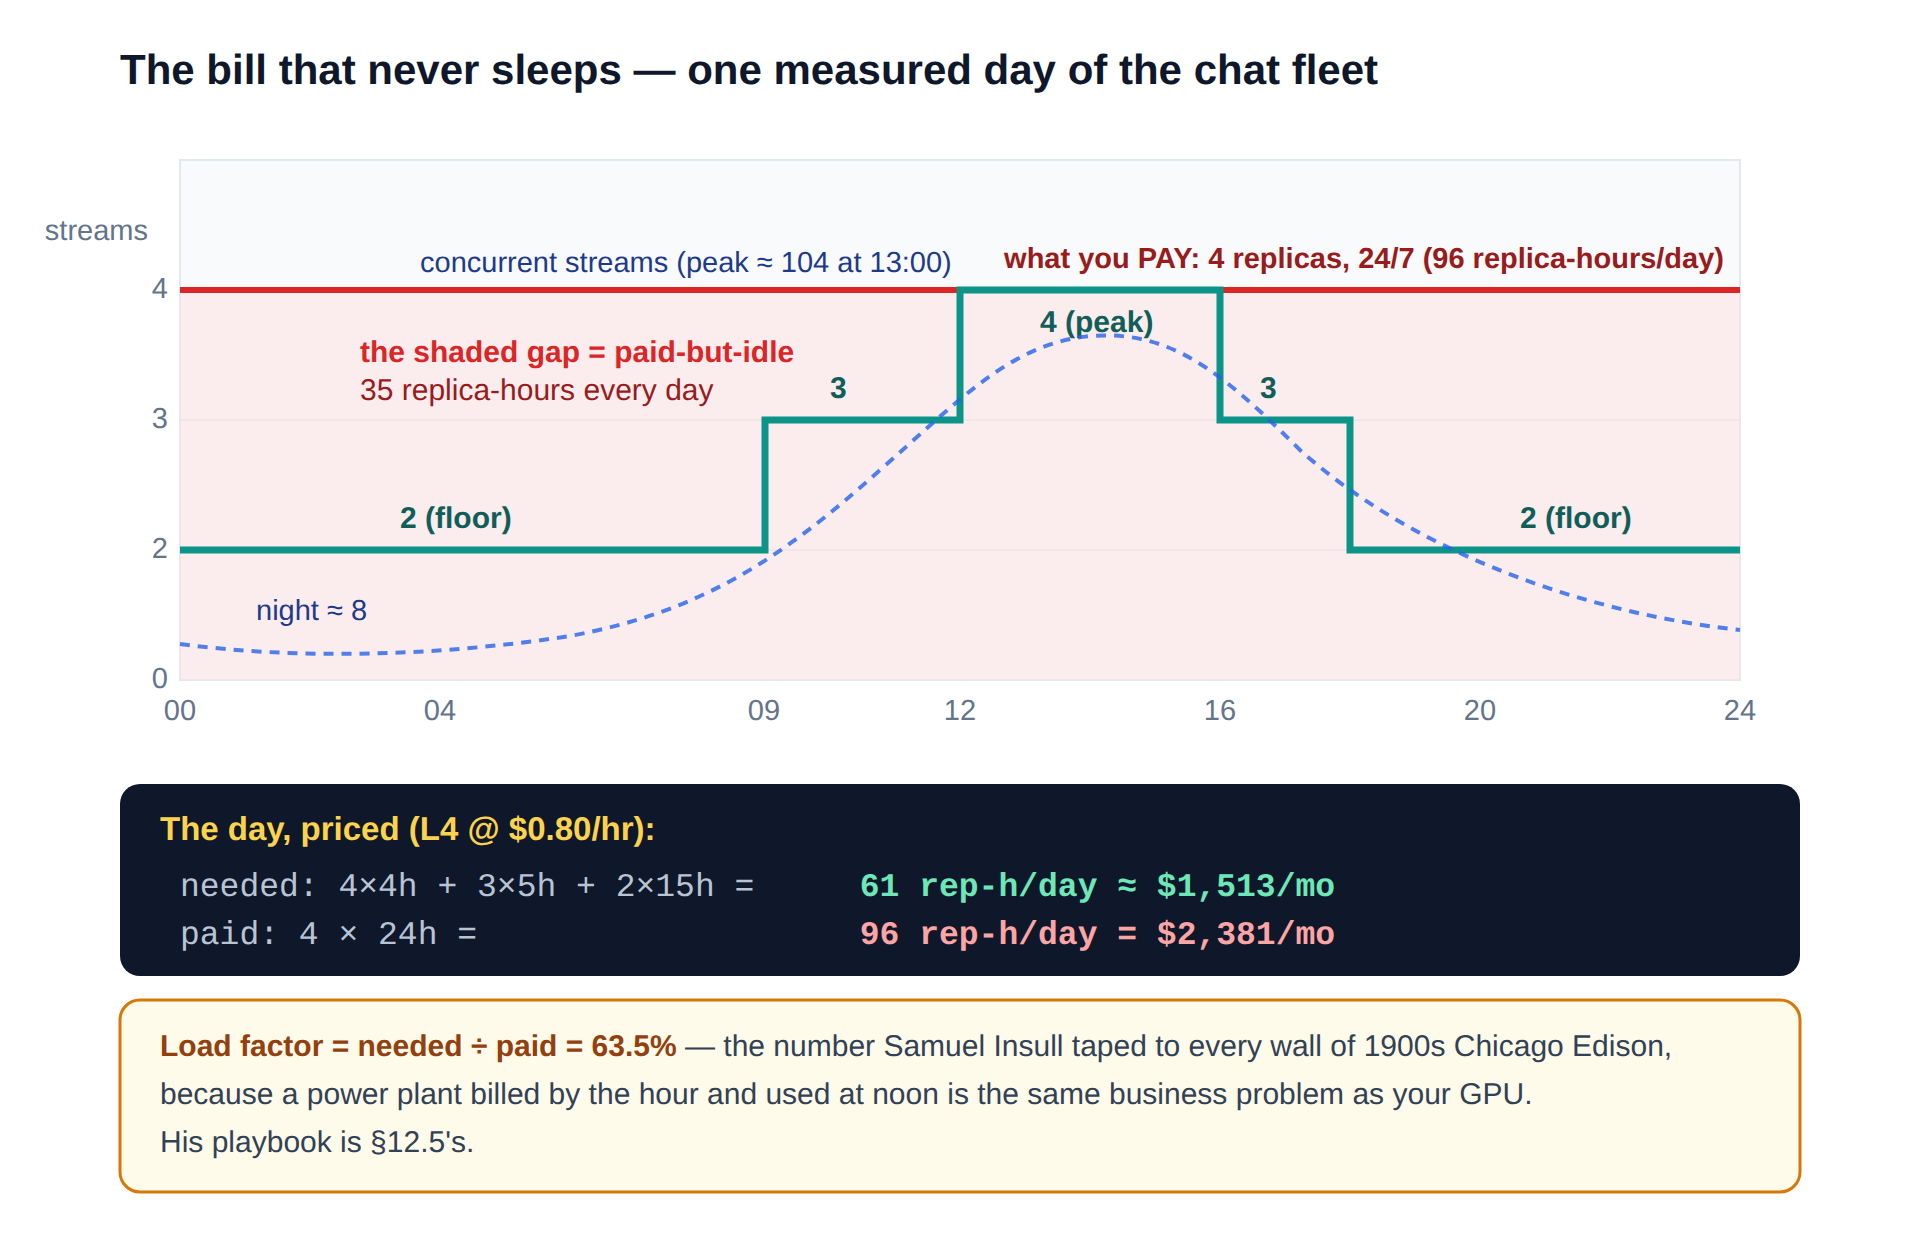
\includegraphics{figures/fig12-1_diurnal.png}}\\[3pt]
  \figcaption{그림 12-1  하루를 그린 모습. 계단은 롤아웃 안전을 위한 바닥 2개를 포함해 SLO가 실제로 요구하는 양이고, 평평한 붉은 선은 정적 플릿이 지불하는 양이다. 그 차이는 매일 야간 근무 35레플리카 시간, 월 \$868다.}
\end{tbbfigure}

\subsection*{1902년: 똑같은 청구서에 직면했던 마지막 산업}

위안이 되는 소식이 있다. 새로운 문제가 아니다. GPU 시간이 아니라 킬로와트시를 팔던 산업이 조부모 세대가 태어나기도 전에 해결했다. 1900년 무렵 전력 회사는 정확히 사례 12-A의 계산 때문에 파산하고 있었다. 발전소는 막대한 고정 비용이 드는데 \textit{저녁 조명 피크에 맞춰 규모를 정하고} 나머지 20시간에는 충분히 쓰이지 않았다. Thomas Edison의 전 비서였고 당시 시카고 전력 회사를 운영하던 \textbf{Samuel Insull}은 수익이 아닌 한 지표에 집착했다. 평균 수요를 최대 수요로 나눈 \textbf{부하율(load factor)}로 사례 12-A 아래쪽과 정확히 같은 비율이다. 전력 회사의 진짜 제품은 \textit{용량}이고 유휴 용량은 순수한 손실이라는 것이 그의 통찰이었다. 골짜기를 채우고 피크를 깎는 게임이다. 그의 회사는 전체 전략을 개척했다. \textbf{소비량뿐 아니라 수요를 계량}했다. 고객의 피크가 발전소 크기를 정하므로 청구서도 피크가 정해야 했으며, 클라우드 가격의 조상이다. \textbf{피크가 서로 맞물리는 고객을 유치}했다. 낮에는 전차, 저녁에는 조명, 밤에는 제빙소와 공장을 운영해 발전소 하나가 세 수요 곡선을 처리했다. 작업을 골짜기로 옮길 수 있는 사람에게 \textbf{비혼잡 시간 전력을 저렴하게 판매}했고, 피크에 공급을 끊어도 되는 산업 고객에게 \textbf{중단 가능 요금}을 제공했다. 전기는 20년 안에 킬로와트시당 약 20센트였던 사치품에서 몇 센트 수준으로 내려왔다. 주된 이유는 더 좋은 발전기가 아니라 더 나은 \textit{부하율}이었다. 이 장의 모든 메커니즘인 오토스케일링, 0으로 스케일링, GPU 공유, 스팟 인스턴스, 야간 배치 기법은 Kubernetes 티셔츠를 입은 Insull의 전략이다. §12.5에서는 당시 고객이 전력을 샀던 방식 그대로 용량을 구매한다.

\subsection*{뻔한 해결책이 두 매복을 만나다}

"수요에 맞춰 레플리카 수만 바꾸면 된다"는 해결책은 기계적으로 모욕적일 만큼 쉽다. 제5장도 이를 약속했다. 오토스케일러는 정수 하나를 수정하는 \textit{원하는 상태의 또 다른 작성자}이고 나머지는 컨트롤러가 모두 처리한다. 흥미로운 엔지니어링은 쉬운 버전이 실패하는 두 방식에 있다. 사례 12-B가 둘을 모두 보여 준다.

\begin{terminalbox}
\begin{Verbatim}[breaklines=true,breakanywhere=true,fontsize=\small,formatcom=\color{tbbtermfg},codes=\tbbcodeactive]
# attempt 1, monday: the tutorial default.
$ kubectl autoscale deploy/chat --cpu-percent=70 --min=2 --max=6
$ kubectl get hpa chat -w              # tuesday, 09:00 wave arrives
NAME   REFERENCE     TARGETS       MINPODS  MAXPODS  REPLICAS
chat   deploy/chat   cpu: 9%/70%      2        6        2
# GPUs drowning (queue growing, TTFT p99 6.1s). CPU: napping at 9%.
# verdict: "9% < 70%, all quiet." it will NEVER scale. wrong eye.

# attempt 2, wednesday: right metric (KEDA on the vLLM queue).
09:00:15  waiting=41 -> desired 2->4       # right eye reacts in 15 s
09:00:24  2 pods Pending -> Init -> ...
09:02:54  ...Ready                         # cold start: 2.5 minutes
# 09:00-09:03: TTFT p99 red. right metric, LATE muscle.
# lesson 1: scale on what users feel. lesson 2: reaction time
# is part of capacity. the wave does not wait for your pods.
\end{Verbatim}
\end{terminalbox}
\figcaption{사례 12-B  아침마다 한 번씩 일어난 두 실패. CPU 기반 오토스케일러는 GPU의 바쁨을 볼 수 없어 전혀 작동하지 않는다. 대기열 기반 오토스케일러는 15초 만에 작동하지만 새 레플리카를 만드는 데 2분 30초가 걸린다. §12.2는 눈을, §12.3은 초시계를 고친다.}

두 매복이 이 장의 뼈대를 만든다. \textbf{§12.2}는 제11장에서 읽는 법을 배운 입장 대기열 지표에 오토스케일러를 연결하고, 목표 공식, 비대칭 안정화 창(stabilization window), 예측 가능한 피크를 위한 예약 증가라는 제어 루프의 실제 조절점을 다룬다. \textbf{§12.3}은 2분 30초의 탄생을 이미지, 가중치, 엔진, 워밍업으로 세분화하고 2주 차 Firecracker를 다시 불러 업계가 이미 해결한 항목이 무엇인지 설명한다. 이어 완화 사다리를 올라 0으로 스케일링과 그 정직한 틈새에 도달한다. \textbf{§12.4}는 사례 1-B가 드러낸 \textit{또 다른} 낭비인 GPU 한 대를 온전히 쓰기에는 너무 작은 서비스를 공격한다. 시분할, MPS, MIG로 제2장의 카드당 테넌트 하나 규칙을 굽힌다. \textbf{§12.5}는 Insull의 포트폴리오를 클라우드 가격으로 조립한다. 약정 바닥, 온디맨드 어깨, 스팟 버스트, 비혼잡 시간 채우기를 사용해 프로젝트 비용을 \$2,381에서 \textbf{\$877}, 즉 영수증을 근거로 1주 차 상한 아래까지 낮춘다. 측정한 단위 경제성(unit economics)으로 제1장의 자체 구축 대 외부 도입 손익분기점도 마무리한다. \textbf{§12.6}은 강의 계획서가 계속 준비해 온 실습으로, 제시하는 모든 수치가 스윕이나 가격표에 근거하는 팀 프로젝트 중간 점검이다.

\begin{calloutbox}{tbbpurple}{tbbpurplefill}
{\normalsize\bfseries\color{tbbpurple}생각해 보기}\par\vspace{3pt}
\begin{tbbitemize}
  \item 사례 12-A의 바닥은 "롤아웃 안전"을 근거로 레플리카 2개다. 제5장의 롤링 업데이트 메커니즘(maxUnavailable/maxSurge)과 제11장의 스트림을 이용해 논거를 재구성하라. 반대편도 주장하라. 바닥을 1이나 0으로 두어도 정당하려면 트래픽과 사용자에 대해 무엇이 참이어야 하는가?
  \item Insull의 수요 계량기는 총소비량이 아니라 피크를 기준으로 고객에게 요금을 부과했다. 이를 클라우드 GPU 가격에 대응시켜라. 클라우드에서 수요 요금에 해당하는 것은 무엇이며, 시간당 온디맨드 가격은 왜 이미 Insull의 논리를 인코딩하는가? 힌트: 각 가격 모델에서 유휴 위험은 누가 부담하는가?
  \item 사례 12-B의 시도 1도 한 가지 트래픽 패턴에서는 실제로 스케일링한다. 그 패턴을 설명하고 GPU 채팅 서비스에서는 절대 나타나지 않는 이유를 말하라. 제9장의 어느 사례를 거울처럼 뒤집은 모습인지도 제시하라.
  \item 팀원이 max=6과 영구적으로 낮은 목표값, 즉 "하루 종일 더 많은 여유 용량"으로 09:00의 매복을 해결하자고 제안한다. 사례 12-A의 원장을 기준으로 가격을 계산하고 실제로 무엇을 사는지 설명하라. 힌트: 계단을 다시 평평하게 만든다.
\end{tbbitemize}
\end{calloutbox}

\section{오토스케일링: 올바른 지표와 초시계}

신비부터 걷어 내자. 어려운 부분은 이미 제5장에서 해결했다. \textbf{Horizontal Pod Autoscaler}는 15초마다 지표를 읽고, 그 지표를 목표에 맞추려면 레플리카가 몇 개 \textit{있어야 할지} 계산한 뒤 Deployment의 \code{replicas} 필드에 답을 쓰는 제어 루프다. 전체 장치는 \textbf{관찰 → 목표 계산 → 정수 하나 수정}이 전부다. 이후의 스케줄링, 이미지 풀, 가중치 로드, 프로브, Service 구성원 관리는 제5장의 조정 메커니즘이 5주 차부터 지켜 온 약속을 이행한다. §5.2의 생각해 볼 문제는 "오토스케일러 자체가 알아야 하는 것이 얼마나 적은지" 알아보라고 했다. 이제 그 보상을 받는다. 목표 계산은 한 줄이다. \textbf{desired = ceil(current × metric ÷ target)}. 레플리카 두 개가 41개의 대기 요청을 처리하고 레플리카당 목표가 10이면 desired = ceil(2 × 20.5 ÷ 10) = \textbf{5}지만 \code{maxReplicas: 4}에 의해 제한된다. 머신러닝도 예측도 없고 기상학자가 아니라 온도 조절기다. 엔지니어링의 핵심은 공식이 주어진 것으로 보는 두 질문에 있다. \textit{어느 지표}를 사용할 것인가, 그리고 \textit{새 용량이 실제로 얼마나 빨리 도착하는가}다.

\begin{tbbfigure}
  \adjustbox{max width=0.94\linewidth,max totalheight=0.46\textheight}{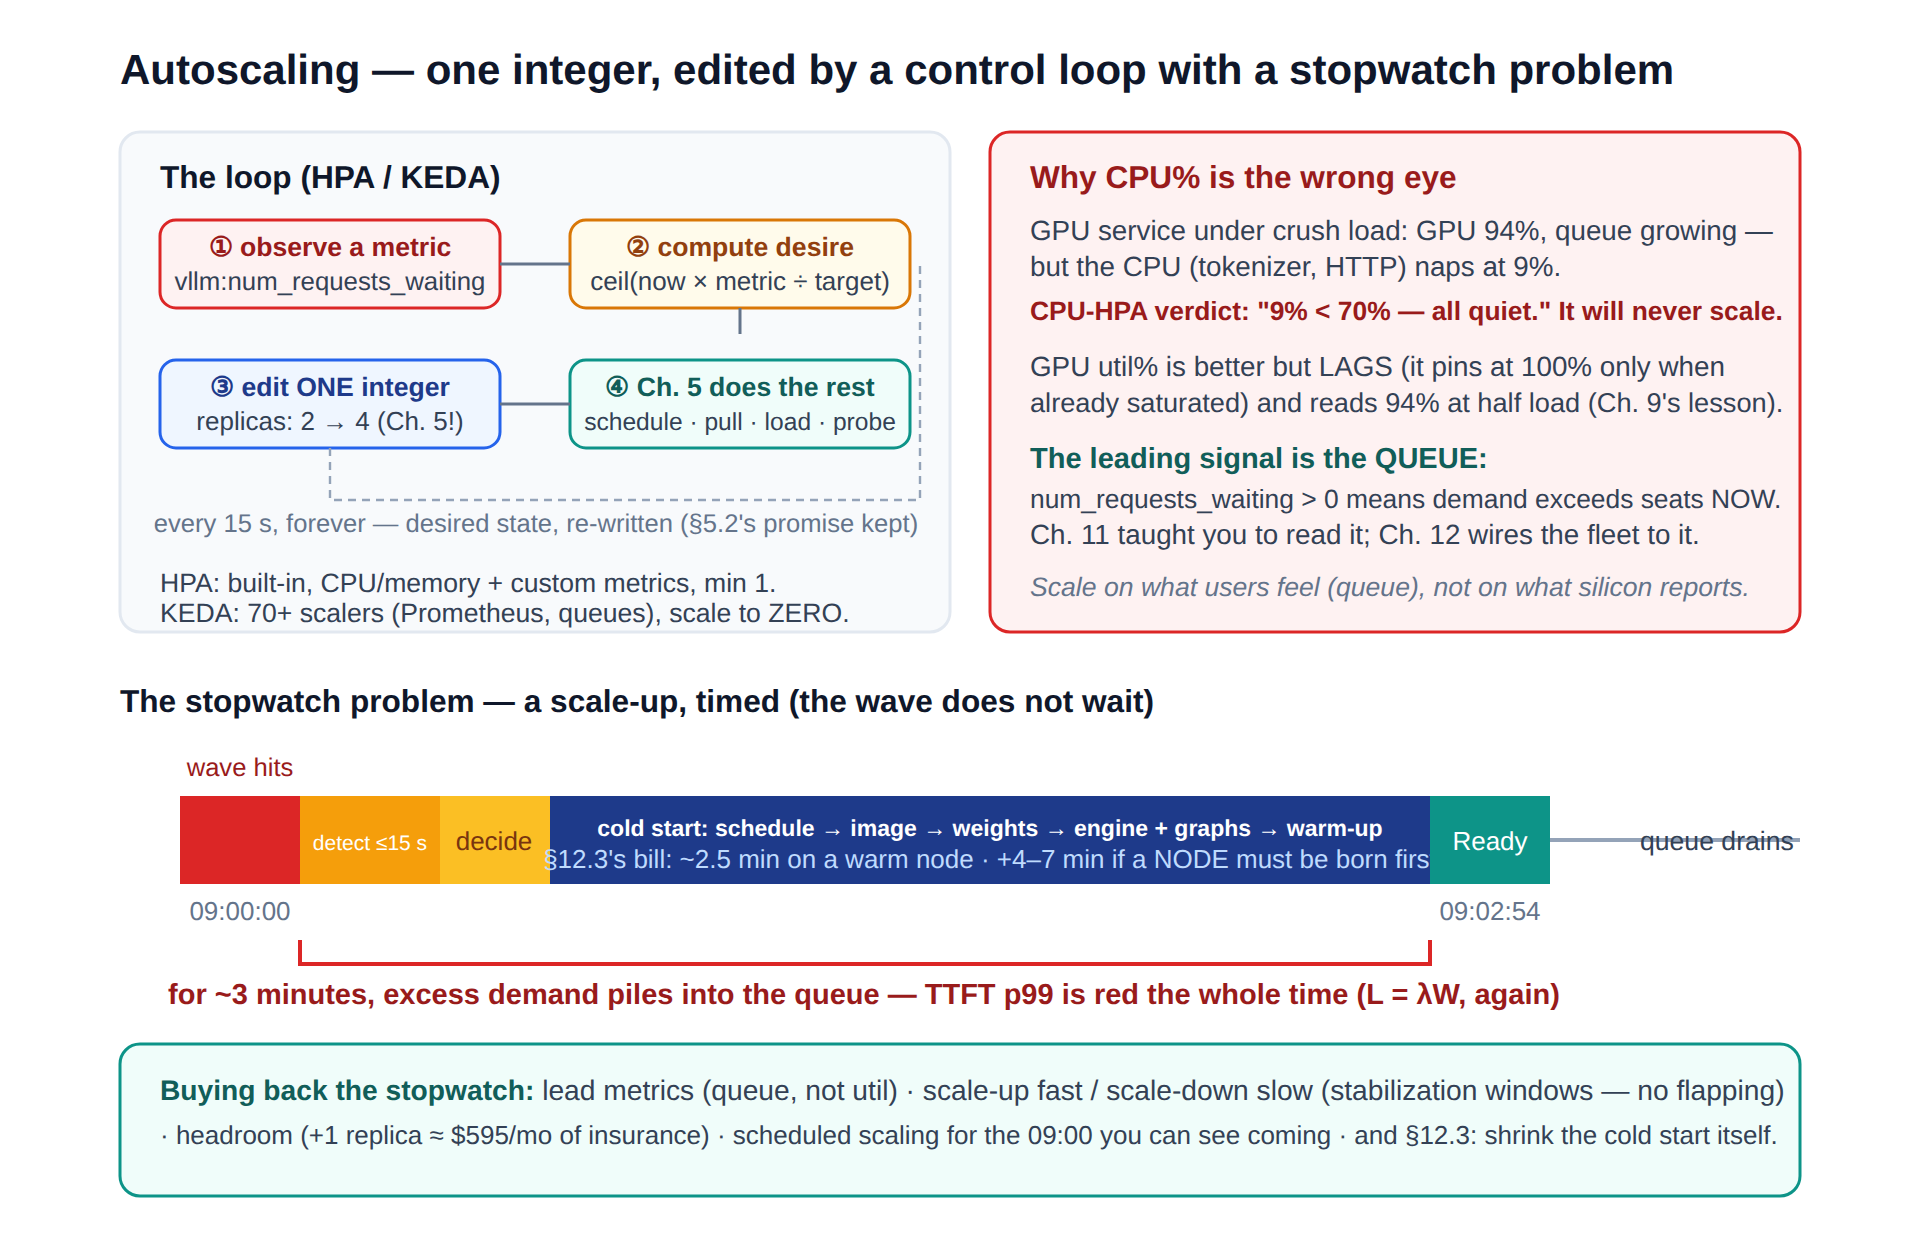
\includegraphics{figures/fig12-2_autoscale.png}}\\[3pt]
  \figcaption{그림 12-2  루프와 두 실패 유형. 왼쪽은 원하는 상태를 수정하는 네 박자 주기이고, 오른쪽은 GPU 서비스에서 CPU\%가 전혀 작동하지 않는 이유다. 아래의 초시계를 보면 감지는 몇 초지만 탄생에는 몇 분이 걸리며 그 차이를 대기열이 먹는다.}
\end{tbbfigure}

\subsection*{눈: 사용자가 느끼는 신호로 스케일링하라}

사례 12-B의 월요일 실패는 논리 오류가 모든 대시보드에서 \textit{보이지 않기} 때문에 분해해 볼 가치가 있다. 기본 HPA는 웹 서버 플릿에서 CPU가 실제 경합 자원이므로 \textbf{CPU\%}를 본다. 채팅 서비스는 구조가 반대다. 제9장 사례 A에서는 GPU가 7\%로 쉬는 동안 CPU가 100\%에 고정되었다. 부하가 걸린 GPU 서비스는 거울상으로, GPU는 94\%인데 토크나이저와 HTTP를 처리하는 CPU는 9\%만 조금 쓰며, 대기열이 끝없이 커지는 동안 CPU만 보는 오토스케일러는 \textit{조용하다}고 결론 낸다. \textbf{GPU 사용률}은 두 번째로 끌리는 선택이지만 두 가지 이유로 역시 틀리다. 먼저 \textit{포화}된다. 카드가 \textasciitilde{}100\%를 표시하면 "수요가 그보다 3× 더 많다"는 사실을 표현할 수 없어 격차가 가장 클 때 오토스케일러가 부족하게 늘린다. 또 \textit{부분 부하에서 거짓말}한다. 제9장에서 커널 실행 병목 서비스는 용량의 절반만 처리하면서도 90\%+를 표시할 수 있음을 배웠다. 올바른 눈은 제11장이 엔진에 넣은 입장 대기열 \textbf{vllm:num\_requests\_waiting}이다. 수요가 좌석을 넘는 순간, 지연 시간 백분위수가 움직이기 전에 0이 아니게 되는 \textit{선행} 지표다. 대기 요청 41개는 용량이 얼마나 틀렸는지 정확히 말하므로 \textit{상한이 없다}. 또한 L = λW에서 대기열은 TTFT의 분자이므로 \textit{사용자가 느끼는 것}이다. 앞으로 작성할 모든 런북(runbook)의 여백에 적을 일반 규칙은 다음과 같다. \textbf{공급 측 게이지(CPU\%, GPU\%, 메모리)가 아니라 수요 신호(대기열 깊이, 진행 중 동시성)로 스케일링하라.} 게이지는 장치가 얼마나 열심히 일하는지 말하고 대기열은 사용자가 얼마나 기다리는지 말한다. SLO는 사용자에 관해 쓴다.

기계적으로 사용자 정의 지표는 두 경로 중 하나로 오토스케일러에 도달한다. \textbf{HPA 경로}는 PromQL을 Kubernetes 사용자 정의 지표 API로 변환하는 지표 어댑터(prometheus-adapter)를 설치한다. 강력하지만 손이 많이 가고 최소 레플리카가 1에서 멈춘다. 실습에서 사용하는 \textbf{KEDA 경로}에서 KEDA는 70개가 넘는 \textit{스케일러}(Prometheus, SQS, Kafka, cron 등)를 갖춘 오퍼레이터이며 CRD 하나로 HPA를 대신 관리한다. HPA와 달리 \textbf{0으로} 스케일링할 수 있다. §12.3에서 0이 왜 전혀 다른 대상인지 설명한다. \code{ScaledObject} 하나가 이 절의 모든 주장을 표현한다.

\begin{terminalbox}
\begin{Verbatim}[breaklines=true,breakanywhere=true,fontsize=\small,formatcom=\color{tbbtermfg},codes=\tbbcodeactive]
apiVersion: keda.sh/v1alpha1
kind: ScaledObject
metadata: {name: chat-scaler}
spec:
  scaleTargetRef: {name: chat}          # the Deployment to edit
  minReplicaCount: 2                    # the floor (rollout safety)
  maxReplicaCount: 4                    # the budget ceiling
  cooldownPeriod: 300                   # scale DOWN slowly (5 min)
  triggers:
  - type: prometheus
    metadata:
      serverAddress: http://prometheus:9090
      query: sum(vllm:num_requests_waiting{app="chat"})
      threshold: "10"                   # tolerate 10 waiting/replica
# scale on the queue users feel - not the CPU nobody uses.
\end{Verbatim}
\end{terminalbox}
\figcaption{기록 12-1  실습의 ScaledObject. 15줄에 올바른 지표(vLLM 입장 대기열), 안전을 위한 바닥, 예산을 위한 상한, 올릴 때는 빠르고 내릴 때는 느린 비대칭 성향이 담긴다.}

\subsection*{성향: 올릴 때는 빠르게, 내릴 때는 느리게}

공식만 사용하면 플릿은 신경질적으로 변한다. 트래픽이 출렁일 때 모든 흔들림을 따라 하는 스케일러는 \textbf{플래핑}한다. 레플리카가 나타나 2분 30초의 탄생 비용을 내고 8분간 서빙한 뒤 죽었다가 다음 흔들림에 다시 태어난다. 청구서 전체를 콜드 스타트 오버헤드로 바꾼다. 제10장의 생각해 볼 문제에서 최악의 특수 사례를 만났다. 스케일 아웃하는 포드마다 도착 시 40초의 torch.compile 워밍업 비용을 내고 매번 p99가 치솟았다. 업계의 해결책은 \textbf{비대칭 안정화}다. 실제 대기열은 평활화를 기다리게 해서는 안 되고 몇 초가 중요하므로 순간 신호에 따라 \textbf{증가}시킨다. \textbf{감소}는 \textit{후행 창의 최악값}을 기준으로만 한다. HPA에서는 \code{scaleDown.stabilizationWindowSeconds: 300}, KEDA에서는 \code{cooldownPeriod}다. 이 비대칭은 CFO에게도 옹호할 수 있는 비대칭 손실 함수를 인코딩한다. 너무 빠르게 늘리면 레플리카 몇 분을 낭비하지만 너무 빠르게 줄이면 다섯 장에 걸쳐 측정한 SLO를 깨뜨린다. 감소 창은 트래픽의 흔들림 주기에 맞춘다. 일중 채팅에는 5분이 적합하고 배치형 트래픽에는 더 길게 둔다. \textbf{바닥}은 부하가 아니라 운영을 기준으로 정한다. 레플리카 두 개면 제5장의 롤링 업데이트 중 하나가 서빙하는 동안 다른 하나를 종료할 수 있다. 바닥이 하나면 모든 배포가 부분 장애가 된다.

\subsection*{초시계: 반응 시간도 용량의 일부다}

이제 수요일의 매복을 보자. 올바른 눈과 차분한 성향이 있어도 루프의 종단 간 반응 시간은 \textbf{T = 감지(≤15 s 지표 스크레이프) + 결정(≤15 s 루프 틱) + 프로비저닝(§12.3의 콜드 스타트: 따뜻한 노드의 포드 \textasciitilde{}150 s, GPU 노드까지 태어나야 하면 6–10 min)}이다. 정직한 경우에도 3분으로 보자. 그동안 \textit{기존} 플릿이 \textit{새} 수요를 흡수하고 대기열이 차이를 적분한다. 09:00의 파도는 좌석 64개에 제공되는 부하를 동시 스트림 64개에서 104개로 올린다. 초당 \textasciitilde{}9건의 턴 도착이 좌석을 찾지 못하고, Ready 시점에는 스트림 약 40개 분량의 수요가 대기열에 모인다. 기록 11-3의 구간 3과 정확히 같고 매일 아침 예약된 시각에 TTFT p99가 붉어진다. 세 가지 해결책을 적용할 순서대로 살펴보자. 볼 수 있는 피크에는 \textbf{예약 스케일링(scheduled scaling)}을 사용한다. 평일마다 09:00에 오르는 트래픽은 예측 문제가 아니라 달력 문제다. 08:40에 바닥을 4로 올리는 KEDA cron 트리거는 40분 × 레플리카 2개 ≈ \textbf{하루 \$1.07}의 비용으로 매복을 없앤다. 볼 수 없는 피크에는 \textbf{여유 용량}을 둔다. 대기 10개 대신 5개를 허용해 목표를 조금 넉넉히 잡거나 영업시간 동안 레플리카 하나를 더 유지하면(\textasciitilde{}\$50/mo) 대기열이 감지 + 탄생 시간을 버틸 시간을 산다. 마지막은 \textbf{탄생 자체를 줄이는 것}이며 다음 절 전체의 주제다. 효과 없는 방법은 루프가 더 빨라지기를 바라는 것이다. 150초 탄생 앞에서 1초 스크레이프(scrape) 간격은 매복을 더 정밀하게 측정할 뿐이다.

\begin{terminalbox}
\begin{Verbatim}[breaklines=true,breakanywhere=true,fontsize=\small,formatcom=\color{tbbtermfg},codes=\tbbcodeactive]
# wednesday again, with the 08:40 cron floor + KEDA queue trigger:
$ kubectl get hpa keda-hpa-chat-scaler -w
TIME      TARGETS        REPLICAS   EVENT
08:40:02  0/10 (cron:4)  2 -> 4     # calendar, not clairvoyance
08:42:33  0/10           4          # 2 births paid BEFORE the wave
09:00:00  wave arrives: streams 64 -> 104
09:00:15  3/10           4          # queue: single digits. absorbed.
09:14:00  peak passes; waiting=0 for 5 min (cooldown)...
09:19:05  0/10           4 -> 3     # reluctant down. no flapping.
# TTFT p99 through the whole event: 0.46 s. the ambush is deleted -
# for $1.07 of pre-warm. compare Exhibit 12-B's three red minutes.
\end{Verbatim}
\end{terminalbox}
\figcaption{기록 12-2  파도를 견딘 결과. cron 트리거가 피크 전에 두 탄생 비용을 내고, 대기열 트리거가 곡선을 처리하며, 쿨다운이 차분하게 감소시킨다. 약 1달러로 사건 내내 SLO를 지킨다. 이 교재가 판매하는 가장 저렴한 보험이다.}

경계를 정직하게 밝히자. 앞의 모든 방법은 \textbf{프로비저닝된 노드 풀 안의 포드}를 스케일링한다. 원하는 포드 수가 노드 용량을 넘으면 \textbf{클러스터 오토스케일러}가 GPU \textit{장치}를 탄생시켜야 한다. 용량 찾기, 부팅, 드라이버 설치에 3–7분이 걸리며 때로는 "no capacity in zone"으로 끝난다. GPU 부족은 실제 날씨와 같고 제2장의 할당량 실습은 온화한 예고편이었다. 수치에서 운영 규칙이 나온다. \textbf{포드는 파도를 쫓고 노드는 예측을 따른다.} 하루의 노드 범위, 즉 계단의 최댓값을 미리 프로비저닝하고 그 안에서 포드 오토스케일링이 숨 쉬게 한다. 노드 오토스케일링은 느린 하루의 조수로 다뤄야 하며 09:00 파도와 TTFT 조항 사이에 세워서는 안 된다.

\begin{calloutbox}{tbbpurple}{tbbpurplefill}
{\normalsize\bfseries\color{tbbpurple}생각해 보기}\par\vspace{3pt}
\begin{tbbitemize}
  \item 기록 11-3의 구간 3(running 32, waiting 26, 레플리카 하나, target 10)에 목표 공식을 적용하라. HPA는 몇 개를 요청하고 maxReplicas는 어디에서 제한하는가? §11.3의 좌석 계산으로 그 상한이 옳은지 판단하고, 이를 높이려면 어떤 예산 수치가 정당화해야 하는지 설명하라.
  \item 트래픽에는 예측 가능한 09:00 증가와 예측할 수 없는 소셜 미디어 스파이크(90초 안에 3×, 10분 뒤 사라짐)의 두 피크가 있다. 둘을 위한 트리거 집합(cron + 대기열 + 여유 용량)을 설계하라. 의도적으로 희생하는 스파이크와 그것이 CFO와 나눌 올바른 대화인 이유도 밝히라.
  \item 팀원이 "더 빨리 비용을 아끼기 위해" scaleDown 안정화를 30 s로 설정한다. 약 7분마다 피크가 오는 출렁이는 트래픽 한 시간을 모델링하라. 탄생 횟수를 세고 각각 150 s인 콜드 스타트 오버헤드 가격을 계산해 "절감"이 음수임을 보인 뒤, 팀원이 옳아지는 트래픽 패턴을 찾아라.
  \item 제5장의 용어인 롤링 업데이트, maxUnavailable, 프로브 게이팅만 사용해 비용 검토자에게 바닥 2개를 옹호하라. 이어 바닥의 월 비용을 계산하고 이를 1로 낮출 수 있는 제품 결정 하나를 제시하라.
\end{tbbitemize}
\end{calloutbox}

\section{콜드 스타트와 0으로 스케일링}

오토스케일러의 힘은 레플리카가 태어나는 속도만큼만 빠르다. 이 절에서는 제7장이 지연 시간에 했던 일을 콜드 스타트에 적용한다. \textbf{하나의 수치로 취급하지 않고 청구 항목으로 세분화한다.} 지난 아홉 장 동안 항목을 하나씩 모았다. 제4장은 이미지 풀의 가격을 계산했고, 제6장은 가중치 로딩 막대를 만들며 "12주 차가 이 막대를 두고 싸운다"고 경고했다. 제10장은 런타임 컴파일 비용을, 제11장은 엔진의 KV 풀 할당과 CUDA 그래프 캡처를 추가했다. 포드 하나가 이 모든 비용을 한꺼번에 내는 모습을 보자.

\begin{terminalbox}
\begin{Verbatim}[breaklines=true,breakanywhere=true,fontsize=\small,formatcom=\color{tbbtermfg},codes=\tbbcodeactive]
$ kubectl describe pod chat-7f9b4-x2kkj | grep -A2 Events; kubectl logs -f ...
09:00:24  Scheduled    assigned to node gpu-pool-b7   #     +2 s
09:00:26  Pulling      image "registry/chat:v9"
09:00:42  Pulled       3.1 GB in 16.1 s               # Ch. 4's slim image,
                                                      # warm node layer cache
09:00:44  vllm  INFO   Fetching weights: 16-way ranged GET
09:00:53  vllm  INFO   6.02 GiB in 8.9 s              # Ch. 6's loader
09:02:28  vllm  INFO   engine init: VRAM load, KV pool alloc,
                       CUDA graph capture... 95 s     # Ch. 11's engine
09:02:54  Ready        readiness probe passed          # after 26 s of
                                                      # scripted warm-up
# total: 150 s. the pod path. if a NODE had to be born first:
# +3-7 min (VM provision, boot, driver install) - and sometimes
# "no capacity in zone." never put a node birth on the SLO path.
\end{Verbatim}
\end{terminalbox}
\figcaption{기록 12-3  한 번의 탄생을 항목별로 나눈 결과. 모든 줄에 해당 장이 있다. 16초 풀은 제4장의 엔지니어링, 9초 가중치 가져오기는 제6장, 95초 엔진 초기화는 제11장이다. 합계 150초는 §12.2의 초시계 문제를 정량화한다.}

\begin{tbbfigure}
  \adjustbox{max width=0.94\linewidth,max totalheight=0.46\textheight}{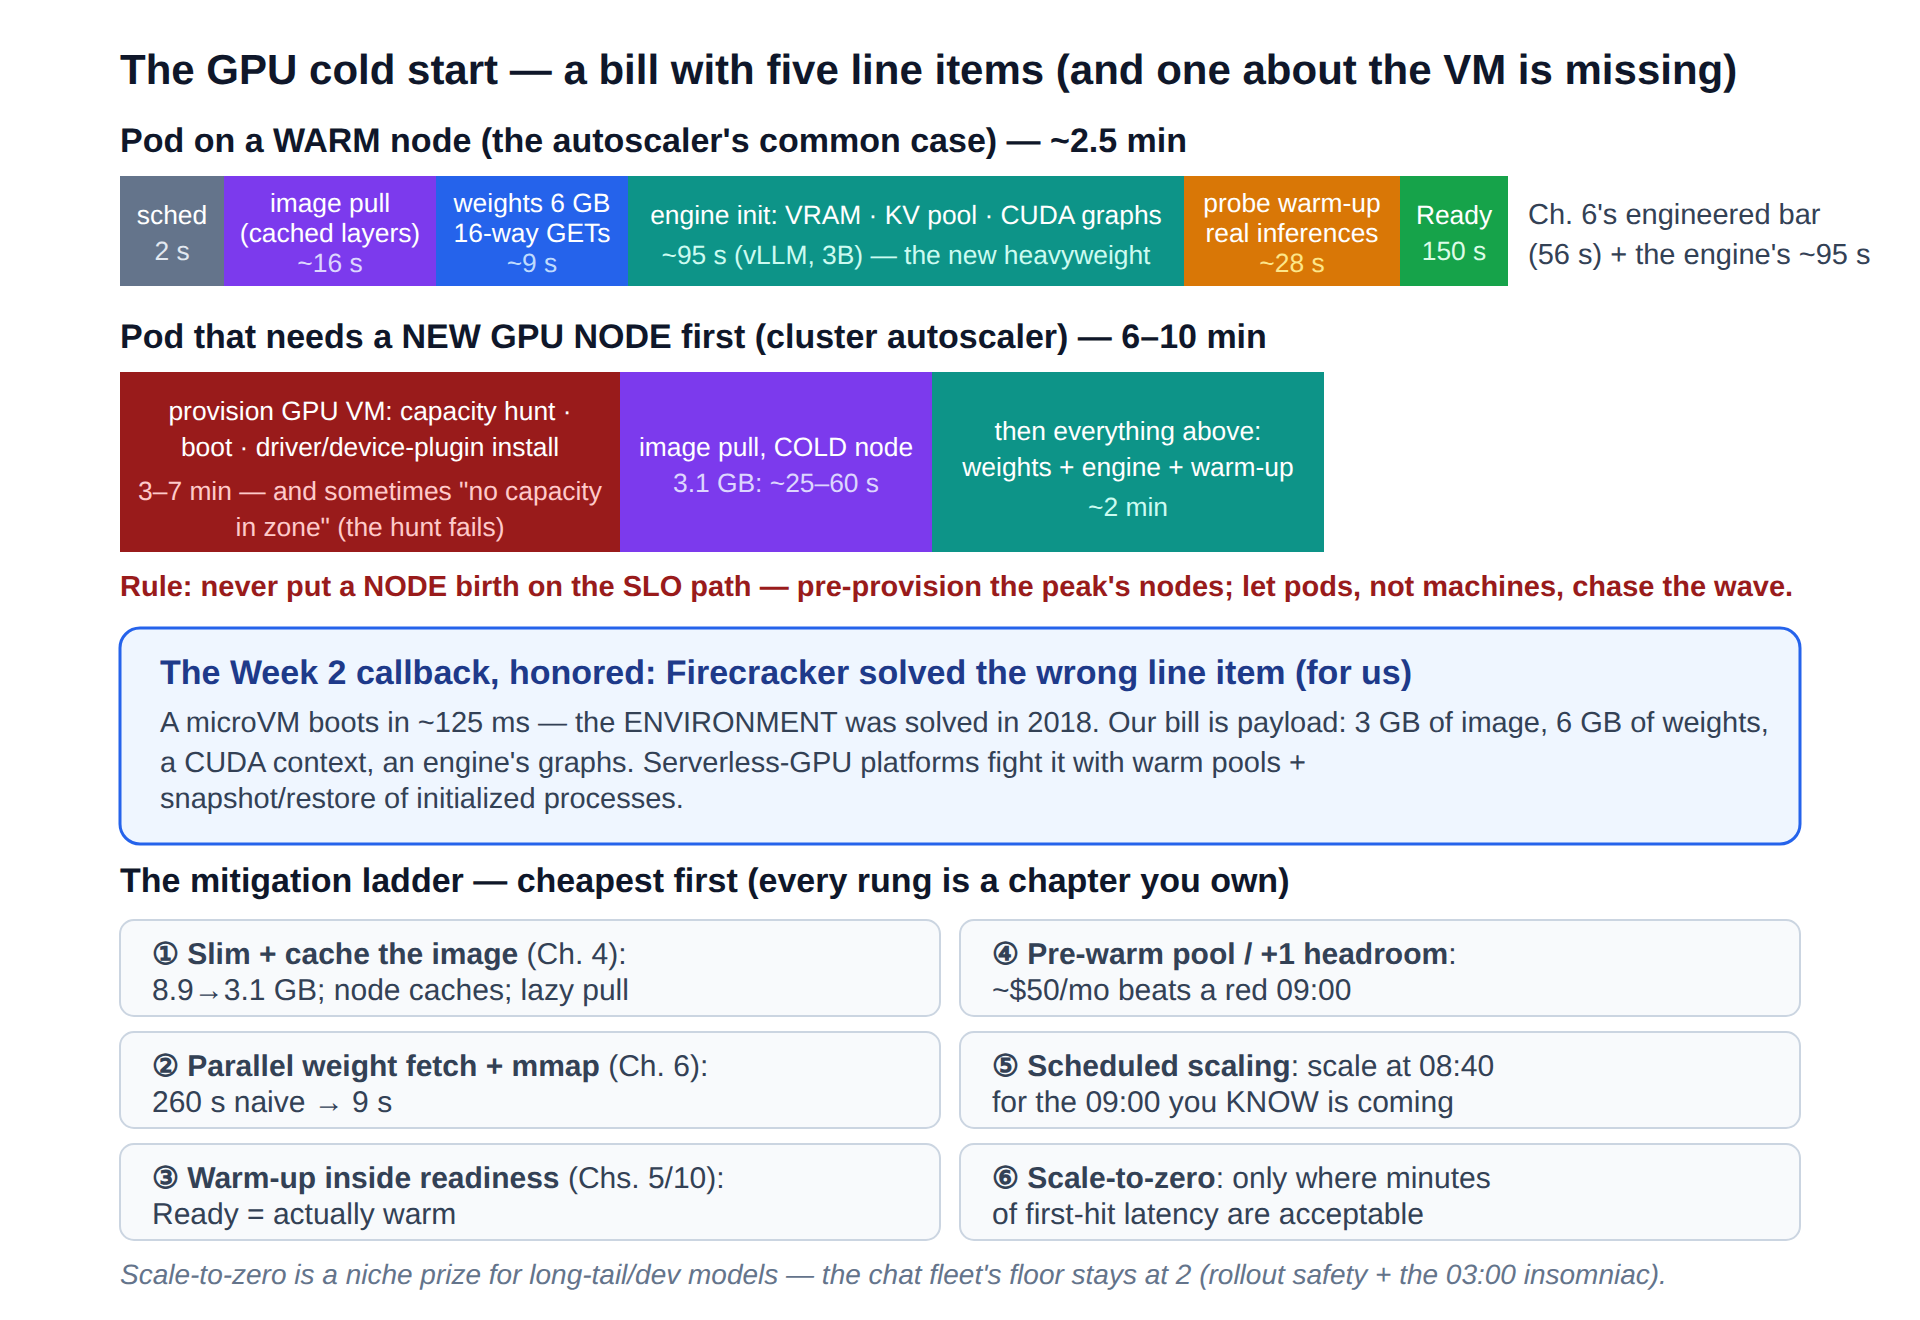
\includegraphics{figures/fig12-3_coldstart.png}}\\[3pt]
  \figcaption{그림 12-3  청구서, 두 경로, 완화 사다리. 따뜻한 노드의 포드는 \textasciitilde{}2.5분이 걸리고 이제 엔진 초기화가 지배한다. 노드 경로는 이를 몇 배로 늘린다. 완화 사다리의 각 단은 이미 이 교재에서 배운 한 장에 해당한다.}
\end{tbbfigure}

\subsection*{다시 등장한 Firecracker — 해결했지만 엉뚱한 항목}

2주 차에 심어 둔 약속을 이제 지켜야 한다. Firecracker의 microVM은 \textbf{\textasciitilde{}125 milliseconds}에 부팅한다. 2005년에 몇 분 걸리던 격리 환경은 2018년에 사실상 공짜가 되었다. 제2장 §2.4는 12주 차의 교훈을 미리 말했다. \textit{"병목은 환경이 아니라 페이로드가 되었다."} 기록 12-3을 이 주장에 비추어 읽어 보자. VM/컨테이너 메커니즘은 2초짜리 \code{Scheduled} 줄에 기여하고 나머지는 거의 없다. 남은 148초는 \textbf{페이로드}다. 3.1 GB 이미지, 6 GB 가중치, CUDA 컨텍스트, 엔진 전체의 할당과 그래프 캡처가 차지한다. 서버리스 CPU는 영리한 문제였지만 \textbf{서버리스 GPU}가 진짜 어려운 이유다. Lambda의 기법인 미리 부팅한 microVM 풀 + 스냅샷/복원은 밀리초 규모 문제를 공격한다. GPU 버전은 \textit{기가바이트}를 미리 배치하고 초기화된 CUDA 프로세스를 되살려야 한다. 초 단위 GPU 요금을 파는 플랫폼(Modal, RunPod, Cloud Run GPU)은 따뜻한 풀, 공격적 이미지 스트리밍, 점차 늘어나는 \textbf{GPU 체크포인트/복원}으로 바로 이 전쟁을 치른다. 완전히 초기화한 엔진 프로세스를 스냅샷하고 몇 초 안에 복원한다. 이 장의 더 읽을거리에 있는 "1초 미만 콜드 스타트" 엔지니어링 글은 모두 이 기법의 변형이다. 가격표를 보면 전쟁이 공짜가 아님을 알 수 있다. 초 단위 요금은 원시 VM보다 프리미엄이 붙는다. 교재의 플릿에는 이런 플랫폼이 아니라 사다리가 필요하다.

\subsection*{완화 사다리 — 0이 차지하는 정직한 틈새}

그림 12-3의 사다리를 가장 저렴한 단부터 오르면 이미 모든 단을 보유했음을 알 수 있다. \textbf{① 이미지 위생}(제4장): 따뜻한 노드 캐시가 있는 다단계 3.1 GB 이미지는 16 s가 걸렸지만 단순한 8.9 GB 이미지는 1분이 걸렸다. 지연 풀 스냅샷터(eStargz, 이미지 스트리밍)는 이미지가 모두 도착하기 전에 컨테이너를 시작한다. \textbf{② 가중치 물류}(제6장): 16방향 범위 GET + safetensors mmap은 260 s를 9초로 줄였다. 노드 로컬 캐시는 같은 노드의 \textit{두 번째} 탄생을 디스크 읽기로 바꾼다. \textbf{③ 준비 상태 안의 워밍업}(제5/10장): 프로브가 스크립트로 추론을 실행해 \code{Ready}가 \textit{따뜻함}을 뜻하게 한다. 피할 수 없는 작업이지만 올바르게 게이트하면 LB가 차가운 포드로 라우팅하지 않고 제10장의 플래핑이 재발하지 않는다. \textbf{④ 사전 워밍업 여유 용량}(§12.2): 영업시간 동안 레플리카 하나를 더 두는 \textasciitilde{}\$50/mo는 알려진 환율로 탄생 지연 시간을 돈으로 바꾼다. \textbf{⑤ 예약 스케일링}: 08:40 cron으로 수요가 생기기 전에 탄생 비용을 낸다. \textbf{⑥ 0으로 스케일링}: 가장 먼 단이며 전혀 다른 대상이다. 0 이후 \textit{첫} 요청이 150 s 전체, 노드 경로라면 몇 분을 사용자에게 보이는 지연 시간으로 먹기 때문이다. KEDA는 탄생 중 요청을 세워 두는 HTTP 애드온으로 이를 지원하고, Knative는 이를 신념처럼 만들었다. 정직한 결정 규칙은 한 문장이다. \textbf{0으로 스케일링은 호출자가 첫 적중의 몇 분 지연을 감당할 수 있는 엔드포인트에 쓴다.} 주 2회 쓰는 롱테일 내부 모델은 유휴 L4 \$595/mo를 \textasciitilde{}\$3로 줄일 수 있고, 개발 환경과 배치 트리거 스코어러도 해당한다. 채팅 플릿의 바닥은 2로 남는다. 03:00의 불면증 사용자도 돈을 내고, 제5장의 롤아웃에는 짝이 필요하다. 엔드포인트마다 계산하면 플릿은 자연스럽게 나뉜다. \textbf{롱테일은 0, SLO를 지는 헤드는 바닥을 둔다.}

\begin{calloutbox}{tbbpurple}{tbbpurplefill}
{\normalsize\bfseries\color{tbbpurple}생각해 보기}\par\vspace{3pt}
\begin{tbbitemize}
  \item 기록 12-3에서 엔진 초기화(95 s)가 이제 지배적인 항목이다. 제10–11장을 이용해 모델 크기와 함께 증가하는 부분, KV 풀 크기와 함께 증가하는 부분, 고정된 부분을 구분하라. 가장 유망한 공격 두 가지를 제안하고 각각의 절감 시간을 추정하라. 힌트: AWQ 가중치는 1.9 GB이고 CUDA 그래프 캡처 범위를 줄일 수 있다.
  \item 세 엔드포인트에서 0으로 스케일링의 가격을 계산하라. (a) 채팅 플릿, (b) 야간 배치 스코어러, (c) 주 \textasciitilde{}5회 사용하는 내부 RAG 데모다. 각각 유휴 비용 절감액, 첫 적중 지연 시간 비용, 결론을 제시하고 (a)의 결론을 뒤집을 제품 문장을 말하라.
  \item "1초 미만 GPU 콜드 스타트" 블로그 글이 화제가 된다. 이 절을 바탕으로 제목 뒤에서 무엇이 참이어야 하는지 나열하라. 무엇을 스냅샷했는가? 가중치는 어디에 사는가? 따뜻한 풀 비용은 누가 내는가? 벤치마크가 거의 확실히 포함하지 않은 것도 밝히라.
  \item 클러스터 오토스케일러가 피크에 L4에 대해 가끔 "no capacity in zone"을 보고한다. 다른 영역 → 다른 GPU 유형 → 온디맨드→스팟 반전 → 대기열 후 성능 저하로 이어지는 폴백 연쇄를 설계하고, 제5장의 nodeSelector/affinity 메커니즘으로 지금 표현할 수 있는 단계를 표시하라.
\end{tbbitemize}
\end{calloutbox}

\section{실리콘 공유: 시분할, MPS, MIG}

오토스케일링은 \textit{너무 많은 전체 GPU}의 낭비를 고친다. 이 절에서는 반대편의 부끄러운 문제를 해결한다. 제1장이 교재를 시작하며 보여 준 \textbf{사례 1-B의 유령}이다. 사용률 0.2\%로 한 달에 \$779.66가 청구된 A10G는 GPU 한 대를 쓰기에는 너무 작은 서비스가 카드 전체를 소유한 경우였다. 제2장 §2.6은 낭비가 구조적인 이유를 설명했다. GPU는 가상화에 저항하고 VT-x에 해당하는 기능이 없으며 커널이 드라이버 대기열의 작업을 선점할 수 없다. 그래서 클라우드 대여 단위는 \textbf{테넌트 하나, 카드 하나}가 되었다. 패스스루의 깔끔한 격리를 잔혹한 세분성으로 제공했다. 또한 12주 차에 이 규칙을 세 가지로 굽히겠다고 약속했다. 얼마나 많은 격리를 포기해 얼마나 많은 사용률을 회수하는지에 따라 세 방법을 순서대로 살펴보자.

\begin{tbbfigure}
  \adjustbox{max width=0.94\linewidth,max totalheight=0.46\textheight}{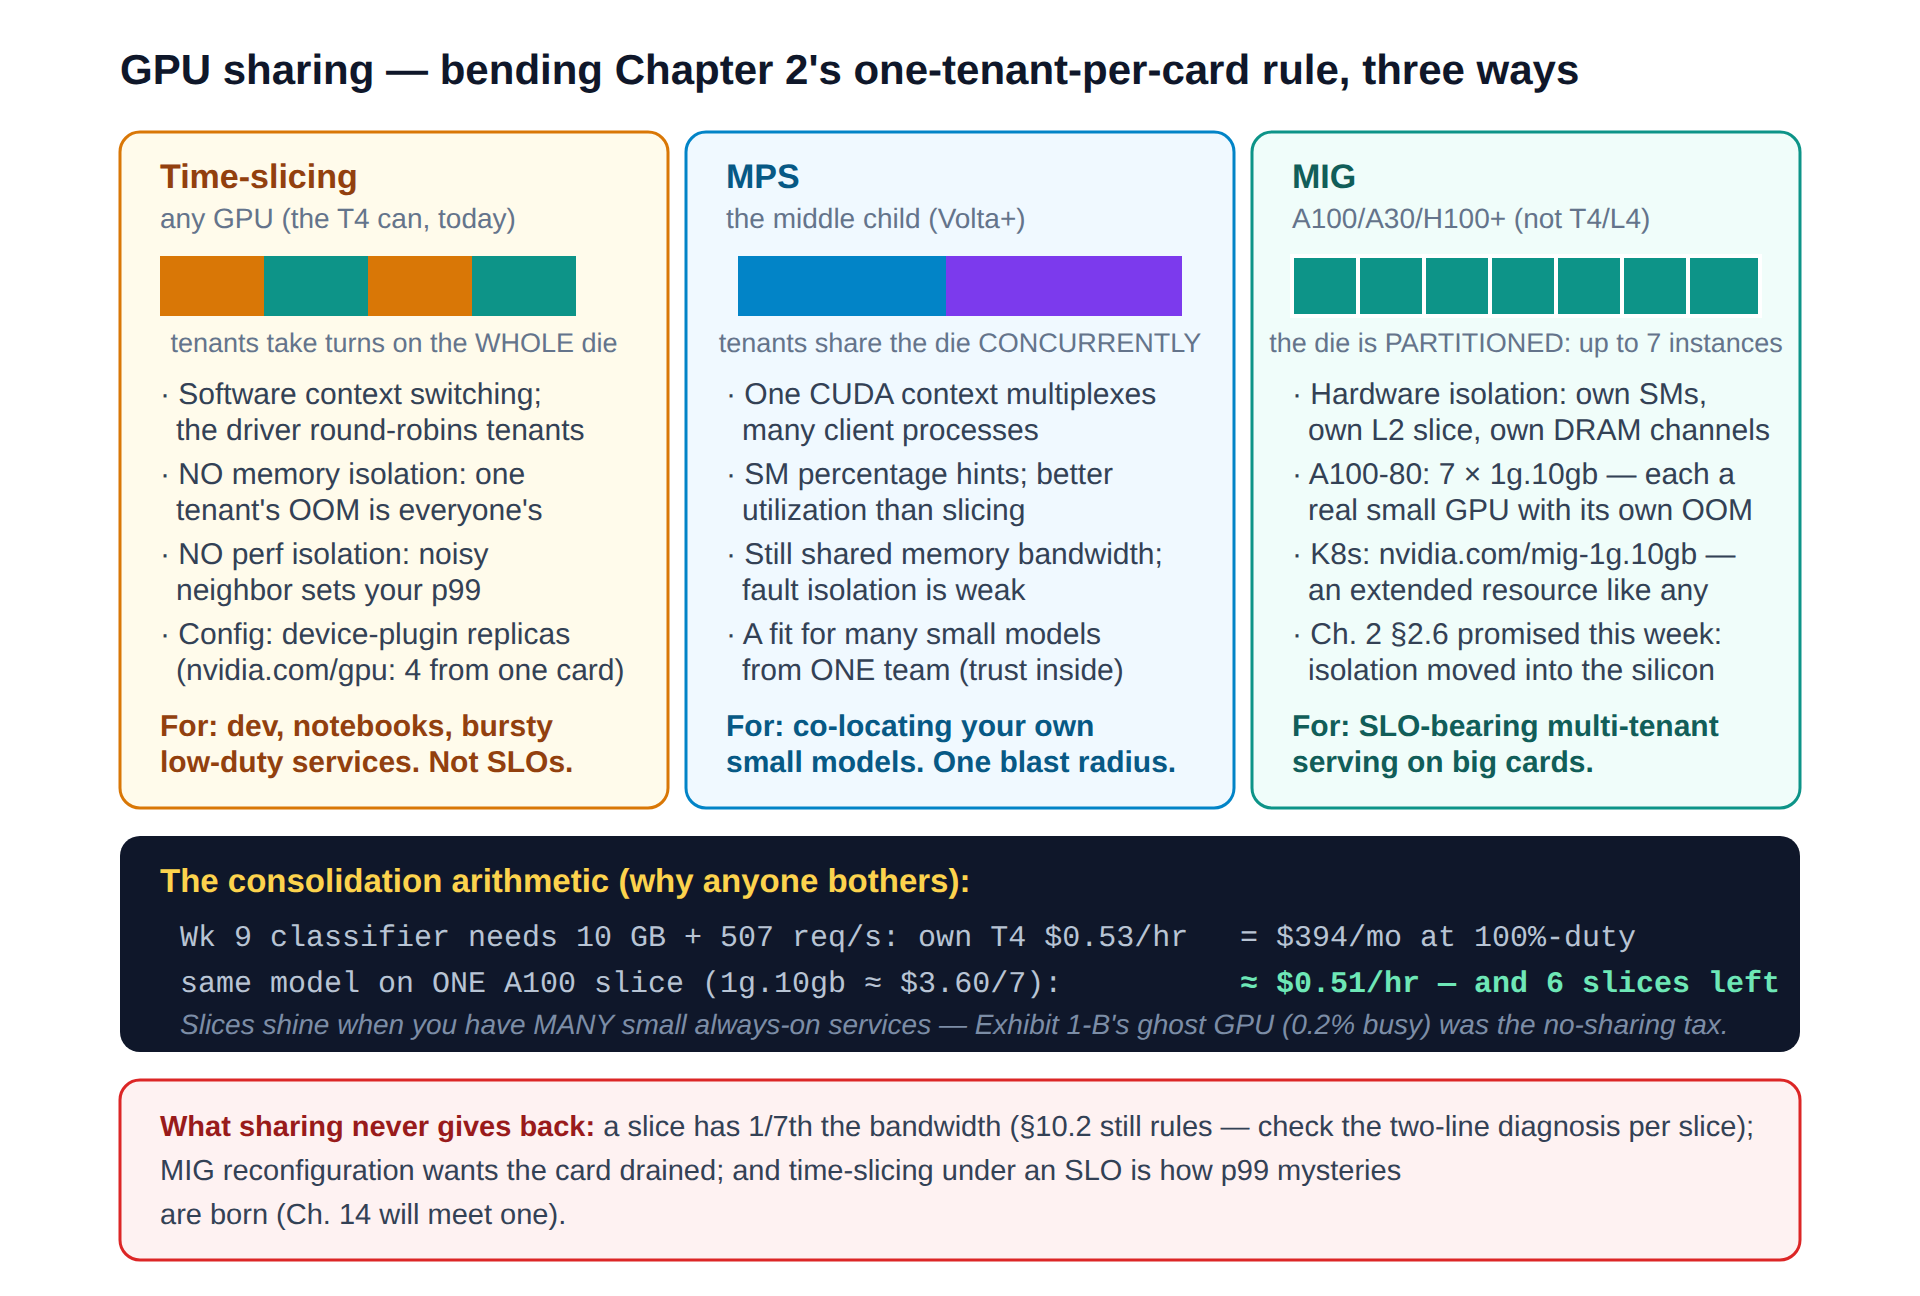
\includegraphics{figures/fig12-4_sharing.png}}\\[3pt]
  \figcaption{그림 12-4  공유의 스펙트럼. 시분할은 전체 다이를 번갈아 쓰며 격리가 없다. MPS는 다이를 동시에 공유하고 장애 반경이 하나다. MIG는 하드웨어에서 다이를 분할해 실제 벽을 만들지만 세분성이 거칠다. 제2장의 규칙을 실리콘 자체가 굽힌다.}
\end{tbbfigure}

\subsection*{시분할: 번갈아 쓰고 정직하게 표시하기}

\textbf{시분할}은 가장 단순하게 규칙을 굽힌다. 1970년대 시분할 운영체제가 CPU 하나를 공유했듯 드라이버가 몇 밀리초씩 테넌트 사이에서 \textit{전체 GPU}의 컨텍스트를 전환한다. Kubernetes는 장치 플러그인 설정으로 이를 연결한다. \code{replicas: 4}를 광고하면 물리 카드 한 장이 \code{nvidia.com/\allowbreak gpu: 4}로 나타나고, 각각 자신이 소유한다고 믿는 포드 네 개를 스케줄링할 수 있다. 어떤 GPU에서도 동작하고 실습의 T4도 포함되며, ConfigMap 하나로 설정할 수 있고 사용률 10\%인 서비스 네 개가 카드 3.6장을 낭비하지 않게 된다. 그 대신 제2장이 패스스루에서 중요하게 본 모든 것을 포기하며 실습에서 이를 \textit{측정}한다. \textbf{메모리 격리가 없다.} VRAM은 먼저 온 사람이 먼저 쓰고 한 테넌트의 누수가 이웃을 OOM으로 만든다. 사례 11-B의 증가가 이제 \textit{공유} 증가가 된다. \textbf{성능 격리가 없다.} 자신의 p99에 이웃의 배치 크기가 들어오고 컨텍스트 전환(context switch) 자체가 모든 테넌트에 비용을 부과한다. \textbf{장애 격리가 없다.} Xid 오류 하나가 모두의 오후를 초기화한다. 정직한 사용 사례는 자연스럽다. 개발 장치, 노트북, 대화형 실험, 모든 이웃이 자기 팀인 사용률 낮은 \textit{내부} 서비스다. 고객 대상 SLO 아래에서 시분할을 쓰면 제14장의 설명할 수 없는 p99 전쟁 이야기가 탄생한다.

\begin{terminalbox}
\begin{Verbatim}[breaklines=true,breakanywhere=true,fontsize=\small,formatcom=\color{tbbtermfg},codes=\tbbcodeactive]
# lab part A-④: slice the T4 four ways, then MEASURE the rent.
$ kubectl apply -f timeslice-config.yaml   # device-plugin: replicas: 4
$ kubectl describe node gpu-node | grep nvidia.com/gpu
  nvidia.com/gpu:  4        # one card, four schedulable "GPUs"
$ kubectl scale deploy/clf --replicas=2    # two classifiers co-tenant

# same sweep as Week 9, alone vs. with a busy neighbor:
            p50      p99      req/s@SLO
alone      2.9ms    9.8ms      507
neighbor   3.1ms   38.4ms      214       # p99 x3.9, capacity /2.4
# nothing is "broken." the card is just honest: two tenants, one die.
# noisy neighbor is not folklore - it is a number you now own.
\end{Verbatim}
\end{terminalbox}
\figcaption{기록 12-4  측정한 공유. 분류기 포드 두 개가 실습 T4를 시분할한다. 각자 실행할 때는 문제가 없지만 함께 실행하면 p99가 네 배가 된다. 제2장이 패스스루로 샀다고 한 격리가 사라지자 그 부재가 보인다. 공유는 실제 할인이지만 실제 대가도 있다.}

\subsection*{MPS와 MIG: 중간 지점과 하드웨어의 답}

\textbf{MPS}(Multi-Process Service)는 중간 단이다. 번갈아 쓰는 대신 테넌트 프로세스의 커널이 공유 CUDA 컨텍스트 하나를 통해 \textbf{동시에} 실행되며, 선택적으로 클라이언트별 SM 비율 상한을 둘 수 있다. 컨텍스트 전환 비용이 없고 유휴 SM이 실제로 이웃 작업을 흡수하므로 사용률은 시분할보다 높다. Volta+부터 주소 공간 격리도 생겼다. 그러나 메모리 대역폭은 여전히 공유하고 장애 반경도 같다. 그래서 MPS는 \textbf{한 팀의 여러 작은 모델}에 가장 적합하다. 자신이 자기 자신의 시끄러운 이웃이므로 스스로 협상할 수 있다. \textbf{MIG}는 제2장 §2.6이 약속한 답이다. Ampere 이후의 큰 다이(A100, A30, H100이며 실습의 T4나 플릿의 L4는 \textit{해당하지 않는다})는 \textbf{하드웨어에서} 최대 일곱 인스턴스로 분할된다. 각각 자체 SM 조각, L2 조각, DRAM 컨트롤러를 가진다. MIG 조각은 진짜 작은 GPU다. 자체 OOM과 장애가 있고, 대역폭은 경합하지 않고 \textit{프로비저닝}된다. 바로 제2장이 표현한 대로 격리가 실리콘 안으로 이동했다. Kubernetes는 각 프로파일을 확장 자원(\code{nvidia.com/\allowbreak mig-1g.10gb})으로 본다. 플릿 설계 질문은 계산 문제가 된다. 9주 차 분류기는 \textasciitilde{}10 GB와 적당한 연산 성능이 필요하다. 전용 T4는 사용률 \textasciitilde{}30\%에서 \$0.53/hr다. \textbf{A100의 1g.10gb 조각 하나는 ≈ \$3.60 ÷ 7 ≈ \$0.51/hr}다. 같은 서비스를 운영하면서 형제용 조각 여섯 개가 남고 유령 GPU 세금을 돌려받는다. 함정은 운영과 §10.2의 모양을 닮았다. 1/7 조각은 \textit{대역폭}도 \textasciitilde{}1/7이므로 조각마다 두 줄 진단을 해야 한다. 얇은 조각의 메모리 병목 모델은 여전히 메모리 병목이다. MIG 구성을 바꾸려면 카드를 드레인해야 하므로 노드 풀별 프로파일을 계획하고 시간마다 바꾸지 않는다. 통합은 \textit{노드} 수준 장애 반경을 집중시킨다. 이제 호스트 하나가 실패하면 서비스 일곱 개가 사라지므로 제5장의 안티어피니티(anti-affinity)가 제값을 한다.

\begin{tbbtablewrap}
  \begin{tabular}{@{}>{\raggedright\arraybackslash}m{\dimexpr 0.1862\tbltextwidth-2\tabcolsep\relax} >{\raggedright\arraybackslash}m{\dimexpr 0.2553\tbltextwidth-2\tabcolsep\relax} >{\raggedright\arraybackslash}m{\dimexpr 0.2606\tbltextwidth-2\tabcolsep\relax} >{\raggedright\arraybackslash}m{\dimexpr 0.2979\tbltextwidth-2\tabcolsep\relax}@{}}
  \arrayrulecolor{tbbnavy}\specialrule{1pt}{0pt}{0pt}
  \rowcolor{tbbtablehead}{\centering \bfseries\color{tbbnavy}모드} & {\centering \bfseries\color{tbbnavy}격리} & {\centering \bfseries\color{tbbnavy}동작 대상 / 세분성} & {\centering \bfseries\color{tbbnavy}정직한 용도} \\
  \arrayrulecolor{tbbnavy}\specialrule{0.7pt}{0pt}{2pt}
  {\textbf{시분할}} & {없음 — VRAM과 장애 공유, 전체 다이를 번갈아 사용} & {모든 GPU (T4 ✓) · 카드당 N개 가상 장치} & {개발, 노트북, 사용률 낮은 내부 서비스 — 고객 SLO에는 사용하지 않음} \\
  \arrayrulecolor{tbbtableborder}\hline
  {\textbf{MPS}} & {동시 커널, SM 상한. 대역폭과 장애 반경 공유} & {Volta+ · 부분 SM 공유} & {한 팀의 여러 작은 모델 — 자신이 자기 이웃} \\
  \arrayrulecolor{tbbtableborder}\hline
  {\textbf{MIG}} & {하드웨어: 자체 SM, L2, DRAM 채널, 자체 OOM} & {A100/A30/H100+ · 최대 7개 조각} & {대형 카드에서 SLO를 지는 멀티테넌트 서빙. 조각 ≈ 작은 GPU} \\
  \arrayrulecolor{tbbtableborder}\hline
  {\textbf{(전체 카드)}} & {패스스루 — 제2장의 깔끔한 기준} & {모든 GPU · 테넌트당 1개} & {플릿의 L4: 카드를 실제로 채우는 인기 모델 하나} \\
  \arrayrulecolor{tbbnavy}\specialrule{1pt}{2pt}{0pt}
  \end{tabular}\par
  \figcaption{표 12-1  공유 결정 요약. 위에서 아래로 읽으며 워크로드가 감당할 수 있는 격리를 제공하는 첫 행을 선택한다.}
\end{tbbtablewrap}

마지막 관점으로 이 절을 장의 주제와 연결해 보자. 공유는 \textbf{Insull의 다양성 기법을 다이 규모에 적용한 것}이다. 그의 발전소는 피크가 맞물렸기 때문에 전차, 조명, 제빙소를 함께 처리했다. MIG로 나눈 A100도 같은 기대를 바탕으로 작은 서비스 일곱 개를 처리한다. 실패 유형도 같다. 피크가 \textit{같은} 고객 일곱을 카드 하나에 넣으면 한 계층 아래에서 13:00 문제를 다시 만든다. 수요의 다양성이 자산이므로 통합하기 전에 측정해야 한다.

\begin{calloutbox}{tbbpurple}{tbbpurplefill}
{\normalsize\bfseries\color{tbbpurple}생각해 보기}\par\vspace{3pt}
\begin{tbbitemize}
  \item 기록 12-4에서 이웃 세금으로 p99는 9.8 → 38.4 ms가 되었지만 p50은 2.9 → 3.1로 거의 움직이지 않았다. 시분할 메커니즘으로 두 수치를 모두 설명하라. 컨텍스트 전환이 운 나쁜 요청과 평균적인 요청에 각각 어떤 영향을 주는가? 평균과 꼬리 중 어느 SLO 조항 형식이 공유를 기만적으로 안전해 보이게 하는가?
  \item 가상의 학과를 위한 MIG 구성을 설계하라. 9주 차 분류기(10 GB, 스파이크형), RAG 임베더(6 GB, 안정적), 내부 요약기(20 GB, 영업시간), 개발 노트북 두 개를 A100-80GB 한 대에 배치한다. 프로파일(1g.10gb/2g.20gb/3g.40gb 혼합)을 고르고 사용 주기로 정당화한 뒤 카드에 넣지 않을 워크로드 하나를 제시하라.
  \item 1g.10gb 조각은 \$0.51로 T4의 \$0.53보다 "유리"하다. 하지만 둘 모두에 §10.2의 같은 두 줄 진단을 적용해 정직하게 다시 비교하라. T4는 320 GB/s, A100의 1/7 조각은 \textasciitilde{}250 GB/s다. 시간당 가격이 아니라 SLO로 결정하라. 언제 T4가 여전히 유리한가?
  \item MPS는 "자신이 자기 자신의 시끄러운 이웃"이라고 설명한다. 자신의 프로젝트에서 피크가 완전히 상관된 같은 트리거의 서비스 두 개로 반례를 구성하고, 피크에는 MPS가 아무것도 절감하지 못하는 이유를 보이라. Insull의 다양성 요구를 CUDA로 다시 표현한 문제다.
\end{tbbitemize}
\end{calloutbox}

\section{KServe와 FinOps 포트폴리오}

두 가지 통합으로 기술 과정이 마무리된다. 하나는 \textit{YAML}, 다른 하나는 \textit{돈}을 위한 통합이다. YAML부터 보자. 이 장에서 설정한 모든 요소를 모델 하나에 적용하면 이제 줄마다 이해하는 약 300줄이 된다. Deployment, 느린 로드를 감싼 프로브(제5장), 저장소 URI에서 모델 가져오기(제6장), 서빙 런타임(제9/11장), Service와 인그레스(제5–6장), 대기열 지표 오토스케일러(§12.2), 적절한 곳에서 0으로 스케일링(§12.3)이 들어간다. 이를 모델 열 개와 팀 세 개로 늘리면 YAML이 스스로 잘못된 내용을 쓰기 시작한다. \textbf{KServe}는 대신 작성해 주는 플랫폼이다. \code{InferenceService} CRD 하나(\textasciitilde{}15줄)에 \textit{모델, 런타임, 오토스케일링 방침, 트래픽 분할}을 선언하면 오퍼레이터가 나머지를 생성한다. 제9장이 KServe를 프레임워크 지도에서 제외하고 다른 종이라고 부른 이유다. \textbf{프레임워크는 "레플리카 하나가 어떻게 잘 서빙하는가?"에 답하고 플랫폼은 "여러 레플리카가 어떻게 살아가는가?"에 답한다.}

\begin{terminalbox}
\begin{Verbatim}[breaklines=true,breakanywhere=true,fontsize=\small,formatcom=\color{tbbtermfg},codes=\tbbcodeactive]
$ kubectl apply -f - <<EOF
apiVersion: serving.kserve.io/v1beta1
kind: InferenceService
metadata: {name: chat}
spec:
  predictor:
    model:
      modelFormat: {name: vLLM}
      storageUri: s3://models/chat/v9-int4/   # Ch. 6's shelf, Ch. 10's gate
    minReplicas: 2
    maxReplicas: 4
    scaleMetric: concurrency                  # §12.2's lesson, built in
    scaleTarget: 28
  canaryTrafficPercent: 10                    # 90/10 split, old/new -
EOF                                           # Chapter 13 drives this knob
inferenceservice.serving.kserve.io/chat created
$ kubectl get isvc chat
NAME   URL                        READY   LATEST   PREV   AGE
chat   http://chat.team.svc...    True    90       10     61s
\end{Verbatim}
\end{terminalbox}
\figcaption{기록 12-5  15줄로 표현한 플랫폼 하나. InferenceService는 이 교재의 제5–12장을 필드로 인코딩한다. canaryTrafficPercent 줄은 제13장을 예고한다. CI 파이프라인이 제어하기를 기다리는 트래픽 분할이다.}

\begin{tbbfigure}
  \adjustbox{max width=0.94\linewidth,max totalheight=0.46\textheight}{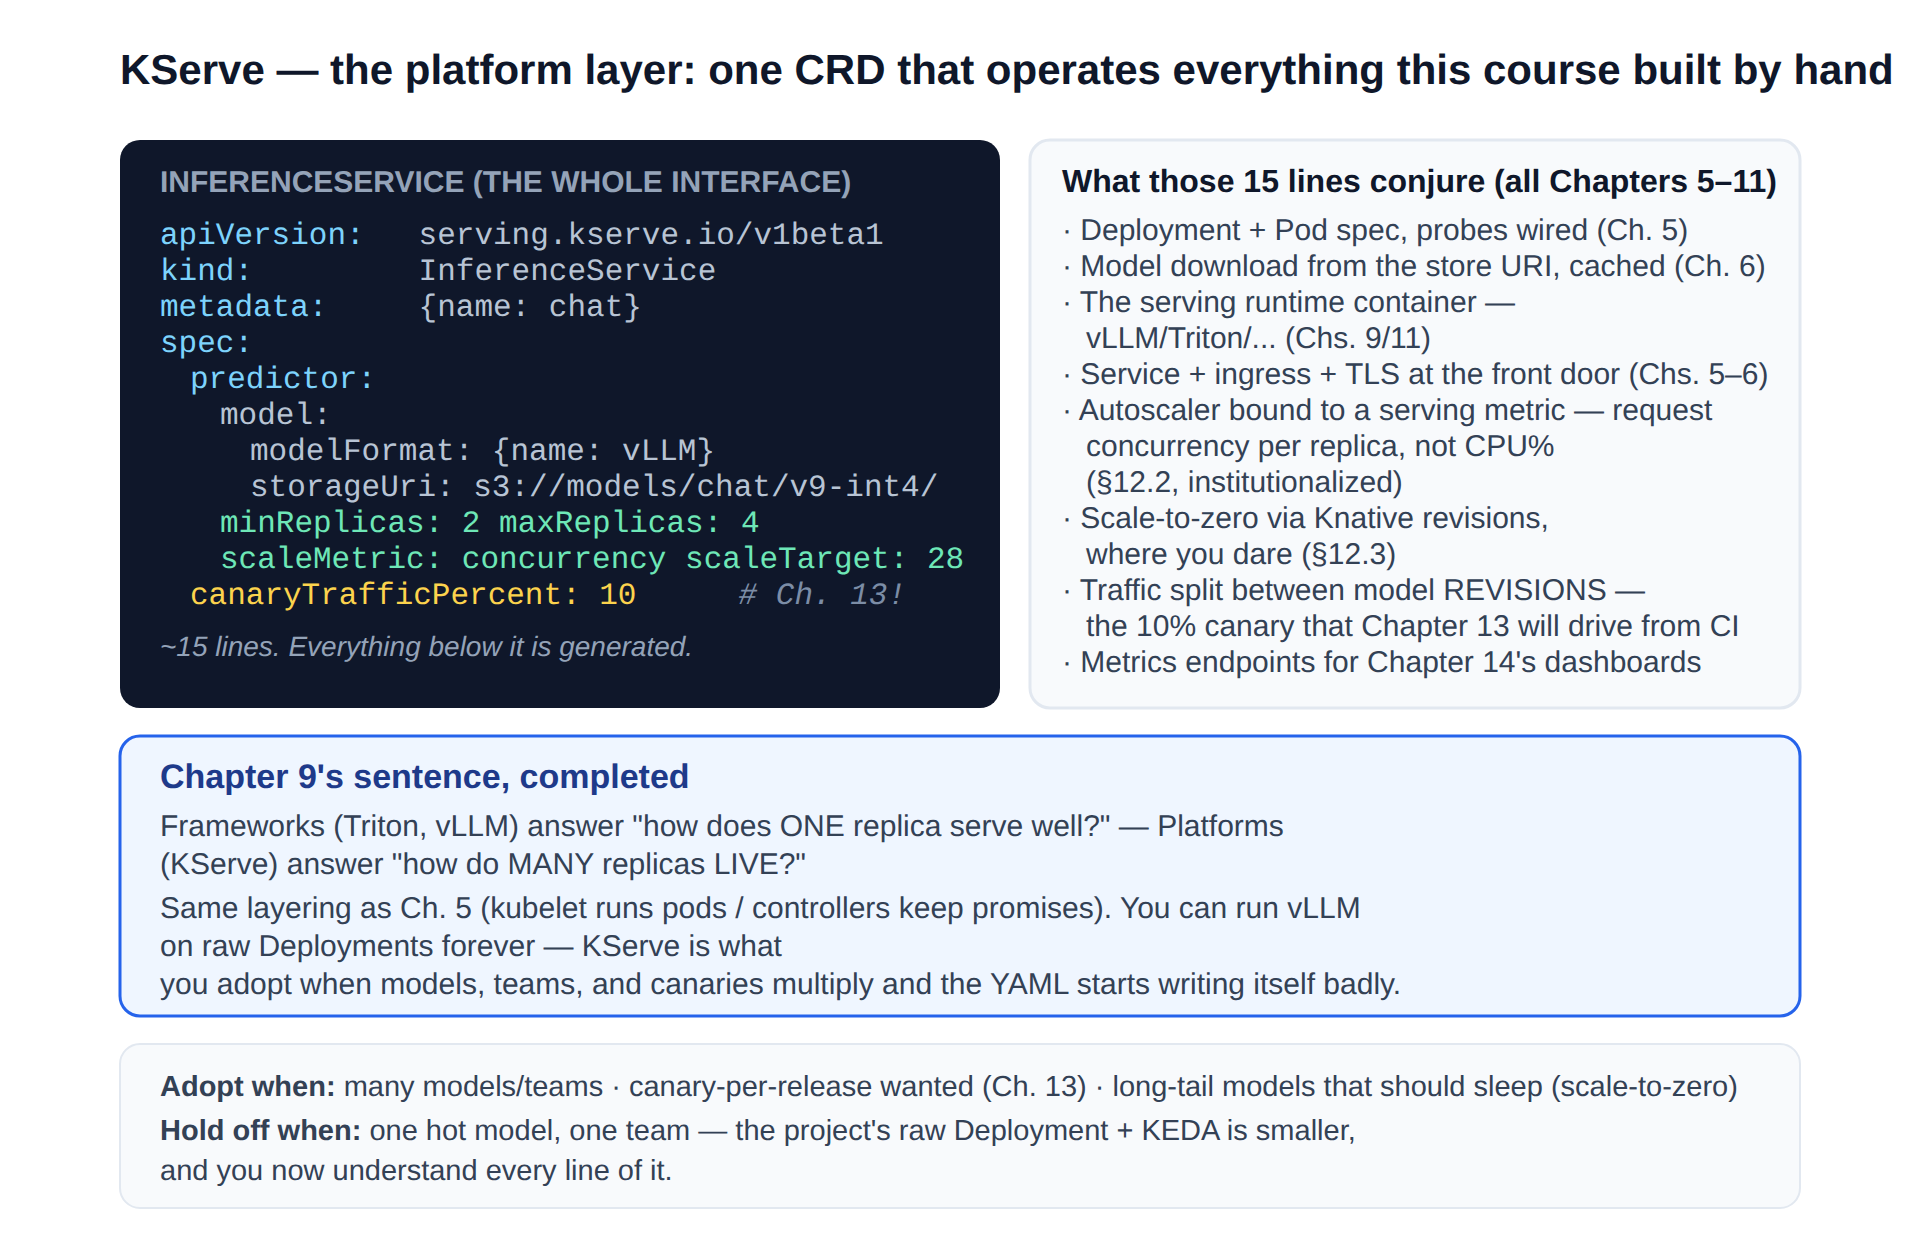
\includegraphics{figures/fig12-5_kserve.png}}\\[3pt]
  \figcaption{그림 12-5  CRD와 CRD가 만들어 내는 것. 모델과 팀이 늘어나면 플랫폼을 도입한다. 인기 모델 하나가 제품 전체라면 원시 Deployment + KEDA를 유지한다. 이제 플랫폼이 대체할 모든 줄을 이해한다.}
\end{tbbfigure}

도입 규칙은 제9장의 프레임워크 조언과 닮아 익숙할 것이다. 여러 모델, 릴리스마다 카나리를 적용하려는 계획(제13장), 잠들어야 할 롱테일 엔드포인트(§12.3)처럼 \textbf{플랫폼의 견해가 잘못 쓰던 YAML에서 구해 줄 때 플랫폼을 도입한다.} 인기 모델 하나가 제품 전체라면 \textbf{도입을 미룬다.} 프로젝트의 원시 Deployment + KEDA가 더 작고 완전히 이해할 수 있으며 의존성도 하나 적다. 관리형 엔드포인트인 SageMaker와 Vertex는 오퍼레이터까지 외주화한 같은 절충이며 제13장에서 다시 다룬다. 어느 쪽이든 KServe가 제도화한 내용에 주목하자. 기본 스케일링 지표는 CPU가 아니라 요청의 \textbf{레플리카당 동시성}이다. §12.2의 주장이 교훈에서 플랫폼 기본값으로 승격되었다.

\subsection*{포트폴리오: Insull이 팔던 방식으로 용량 구매하기}

이제 돈을 보자. 지금까지는 소비하는 레플리카 시간이 \textit{몇 시간}이어야 하는지 적정 규모를 정했다. 마지막 수단은 \textit{각 시간}의 가격을 정하며, 선택지는 Insull의 요금표가 다시 태어난 모습이다. 클라우드가 같은 GPU 시간을 세 가격으로 파는 것은 판매자 관점에서 그와 같은 문제인 유휴 용량을 관리하기 때문이다. \textbf{약정 사용}(1–3년 약정, 30–60\% 할인)은 기본 부하 요금이다. 실행할 것이 확실한 바닥의 유휴 위험을 구매자가 맡아 양쪽 모두 이익을 얻는다. \textbf{온디맨드}(정가)는 부하 추종 요금이다. 약속이 전혀 없고 프리미엄 자체가 \textit{유연성}이다. \textbf{스팟/선점형(preemptible)}(60–90\% 할인)은 말 그대로 중단 가능 산업 요금이다. 클라우드는 피크에 GCP 30초, AWS 2분 전 통보 후 회수할 수 있으며, 할인은 이를 견디도록 엔지니어링한 대가다. 사례 12-A의 계단에서 포트폴리오 규칙이 자연스럽게 나온다. \textbf{바닥은 약정하고, 어깨는 온디맨드로, 버스트는 스팟으로 처리한다. 바닥을 스팟에 두지 않는다.} 03:00의 불면증 사용자에게는 약정한 실리콘이 필요하다. Insull의 기법 하나를 더하면 구성이 완성된다. \textbf{비혼잡 시간 채우기}다. 그의 야간 전력은 제빙소로 갔고 야간 GPU는 제7장의 배치 모드로 간다. 재임베딩 작업, 평가 스윕, 보정 실행처럼 설계상 중단 가능한 작업이 스팟에 가장 잘 맞는다. SLO를 건드리지 않고 부하율을 높인다.

\begin{tbbtablewrap}
  \begin{tabular}{@{}>{\raggedright\arraybackslash}m{\dimexpr 0.2181\tbltextwidth-2\tabcolsep\relax} >{\raggedright\arraybackslash}m{\dimexpr 0.1862\tbltextwidth-2\tabcolsep\relax} >{\raggedright\arraybackslash}m{\dimexpr 0.2766\tbltextwidth-2\tabcolsep\relax} >{\raggedright\arraybackslash}m{\dimexpr 0.3191\tbltextwidth-2\tabcolsep\relax}@{}}
  \arrayrulecolor{tbbnavy}\specialrule{1pt}{0pt}{0pt}
  \rowcolor{tbbtablehead}{\centering \bfseries\color{tbbnavy}계층(전력망의 조상)} & {\centering \bfseries\color{tbbnavy}정가 대비 가격} & {\centering \bfseries\color{tbbnavy}거래 조건} & {\centering \bfseries\color{tbbnavy}교재 플릿에서의 용도} \\
  \arrayrulecolor{tbbnavy}\specialrule{0.7pt}{0pt}{2pt}
  {\textbf{약정(기본 부하)}} & {−30–60\%} & {1–3 yrs의 유휴 위험을 구매자가 부담} & {레플리카 2개의 바닥: 2 × \$595 × 0.60 = \$714/mo} \\
  \arrayrulecolor{tbbtableborder}\hline
  {\textbf{온디맨드(부하 추종)}} & {정가} & {약속 없음. 프리미엄 = 유연성} & {오토스케일러가 추가하고 제거하는 어깨} \\
  \arrayrulecolor{tbbtableborder}\hline
  {\textbf{스팟(중단 가능 요금)}} & {−60–90\%} & {30 s–2 min 전 통보. 드레인을 설계해야 함} & {피크 버스트: 13 rep-h/day × \$0.28 ≈ \$113/mo} \\
  \arrayrulecolor{tbbtableborder}\hline
  {\textbf{비혼잡 시간 채우기(제빙소)}} & {야간 스팟} & {골짜기의 중단 가능한 작업} & {03:00의 배치 재임베딩, 평가, 보정} \\
  \arrayrulecolor{tbbnavy}\specialrule{1pt}{2pt}{0pt}
  \end{tabular}\par
  \figcaption{표 12-2  변환한 요금표. 같은 GPU 시간에 세 가격이 붙으며 유휴 위험을 누가 지고 중단을 누가 견디는지가 다르다.}
\end{tbbtablewrap}

\subsection*{눈물 없이 스팟에서 서빙하기 — 드레인 훈련}

배치뿐 아니라 \textit{서빙}에 스팟을 쓰려면 자격을 얻어야 하며, 그 자격은 이미 가진 조각을 안무하는 데서 나온다. 메타데이터 엔드포인트나 노드 테인트로 중단 통보가 도착한다. 포드의 \textbf{preStop hook + terminationGracePeriodSeconds}가 준비 상태를 바꿔 새 입장을 막고 진행 중 스트림이 끝나게 한 뒤 LB에서 등록을 해제한다. 제5장의 우아한 종료 메커니즘이 마침내 시스템을 지탱한다. 제11장에서 측정한 가장 긴 정직한 스트림 시간이 바로 유예 기간이다. \textbf{상태 비저장은 마지막 배당금을 지급한다}(제6/11장). 끝내지 못한 스트림은 다른 레플리카에서 다시 프리필한다. 짧은 지연 시간 증가일 뿐 잘못된 답은 나오지 않는다. 롤아웃과 접두사 캐시(prefix cache) 미스를 안전하게 만든 같은 성질이다. 스팟 풀은 영역과 인스턴스 유형에 걸쳐 다양화하고 용량 최적화 할당을 사용한다. 폴백도 설정한다. 스팟이 회수되고 대체되지 않으면 오토스케일러가 온디맨드로 격차를 채운다. 한 시간 동안 할인을 잃을 뿐 SLO를 잃지는 않는다. 중단이 지루하게 느껴질 때까지 스테이징에서 훈련한다. \textbf{절대 규칙은 스팟이 바닥이 아니라 버스트 계층이라는 것}이다. 누군가는 언제나 시도하므로 점검표에 위험 신호로 넣었다.

\subsection*{원장을 마감하다 — 제1장의 손익분기점도 함께}

\begin{terminalbox}
\begin{Verbatim}[breaklines=true,breakanywhere=true,fontsize=\small,formatcom=\color{tbbtermfg},codes=\tbbcodeactive]
$ python fleet_ledger.py --final          # the course's bill, walked
 Wk 7  estimated, 8 x L4, 24/7             $4,762   # the syllabus bill
 Wk 10 INT8: 2x goodput -> 4 replicas      $2,381   # same SLO
 Wk 12 autoscale: 61 rep-h/day             $1,513   # same SLO
 Wk 12 portfolio:
   commit floor  2 x $595.20 x 0.60      $  714.24
   spot burst    403 rep-h x $0.28       $  112.84
   pre-warm + cron cushion               $   49.60
   TOTAL                                 $  876.68   < $900 ceiling

 unit economics (measured, Wk 11 sweeps):
   capacity  ~3.1B tok/mo   served ~2.0B tok/mo  (load factor again!)
   $/M tokens: 876.68 / 2000 = $0.44   vs API $0.50: self-host wins
   ...at THIS utilization. at half the traffic, the API wins. Ch. 1's
   break-even curve: closed, with measured numbers, 11 weeks later.
\end{Verbatim}
\end{terminalbox}
\figcaption{기록 12-6  결승선. \$4,762 → \$2,381(최적화) → \$1,513(오토스케일링) → \$877(포트폴리오)로 줄어 1주 차 상한보다 \$23 낮아졌다. 모든 단계가 측정한 수단이다. \$/M-token 항목은 교재 첫머리의 자체 구축 대 외부 도입 질문을 마무리한다. 답은 구호가 아니라 사용률이었다.}

세 가지 습관이 일회성 승리를 영웅적인 오후가 아닌 지속적 규율인 \textbf{FinOps}로 바꾼다. \textbf{총액이 아니라 단위를 계량한다.} 중요한 청구서는 \$/M tokens 또는 \$/K requests다. 주, 모델, API 대안과 비교할 수 있기 때문이다. 총지출은 제품이 성장했다는 사실만 알려 준다. \textbf{태그를 붙이고 비용을 공개한다.} 모든 자원에 team/model/env 레이블을 붙여 원장을 분해한다. 제6장의 NAT 함정(\$5k/yr, 조용함)은 태그 없는 배관에 숨은 지출의 대표 사례다. \textbf{이상에 경보를 건다.} 예측의 80\%/100\%/120\%에서 예산 경보를 울린다. 제2장 실습의 가드레일(guardrail)이 프로덕션으로 승격되어 누수 GPU, 잊힌 개발 플릿, 트래픽으로 청구되는 재시도 폭풍을 잡는다. 화려한 일은 아니지만 \$877이 그대로 유지되는 것과 유령 GPU가 조용히 돌아오는 것의 차이다. 한 세기 뒤에도 Insull의 진짜 제품은 같다. \textbf{감시하는 용량}이다.

\begin{calloutbox}{tbbred}{tbbxFEF2F2}
{\normalsize\bfseries\color{tbbx991B1B}상자 12-1  비용 검토의 위험 신호 — 공개 점검표}\par\vspace{3pt}
\begin{tbbitemize}
  \item \textbf{단위 비용 없음} — \$/M tokens 없이 총지출만 있으면 비용 검토가 아니라 성장 차트다.
  \item \textbf{피크에 맞춘 약정} — 유휴 시간을 다시 산 셈이다. 바닥만 약정하고 나머지는 포트폴리오로 구성하라.
  \item \textbf{바닥에 스팟 사용} — 03:00에 호출하는 할인이다. 버스트 계층에만 쓰고 드레인 훈련을 반복한다.
  \item \textbf{트래픽 그래프의 평평한 레플리카 선} — 사례 12-A는 한눈에 진단할 수 있다. 부하율을 대시보드에 넣어야 한다.
  \item \textbf{태그 없는 지출 / 조용한 배관} — NAT 함정, 잊힌 개발 플릿, 좀비 볼륨이다. 귀속할 수 없으면 검토할 수도 없다.
  \item \textbf{SLO 인용 없이 주장하는 절감} — 줄인 모든 비용은 깨뜨리지 않은 조항을 밝혀야 한다. 이 장은 \textit{같은} SLO에서 비용을 절반으로 줄였으며 그 문장이 규율의 전부다.
\end{tbbitemize}
\end{calloutbox}

\vspace{3.0pt}

\begin{calloutbox}{tbbpurple}{tbbpurplefill}
{\normalsize\bfseries\color{tbbpurple}생각해 보기}\par\vspace{3pt}
\begin{tbbitemize}
  \item 트래픽이 두 배이고(피크 동시 스트림 208개, 같은 형태) 기록 12-6을 다시 작성하라. 계단, rep-h/day, 포트폴리오 분할, 최종 청구서, \$/M tokens를 계산하라. 어느 항목이 개선되고 어느 항목이 나빠지는가? 제품이 성장할수록 단위 비용이 \textit{낮아지는} 이유도 설명하라. Insull이라면 알고 있을 것이다.
  \item 약정은 1년간 레플리카 2개를 포함한다. 4개월째에 INT4 빌드(§11.5)가 도입되어 레플리카마다 스트림을 1.6× 더 처리한다. 과도하게 약정했는가? 성장해 채우기, 바닥 워크로드 이동, 재판매/수정 선택지를 검토하고 최적화 로드맵 아래에서 약정할 계획 규칙을 도출하라.
  \item KServe 카나리 필드는 트래픽을 90/10으로 나눈다. 하지만 §10.3의 게이트는 INT4 모델이 안전하다고 이미 결정했다. 카나리는 게이트가 확인할 수 없는 무엇을 검사하는가? 실제 트래픽 분포, 실제 인프라, 실제 SLO를 고려하라. 제13장의 첫 논거를 세 문장으로 작성해 보라.
  \item 실습 원장에서 자신의 프로젝트 손익분기 API 가격을 계산하라. 어느 \$/M tokens에서 자체 호스팅의 우위가 사라지며, 사용률, GPU 가격, 레플리카당 토큰 중 어느 단일 입력이 답을 가장 크게 움직이는가? "왜 그냥 API를 쓰지 않는가?"에 답하는 한 장짜리 슬라이드로 제시하라.
\end{tbbitemize}
\end{calloutbox}

\section{실습: 프로젝트 중간 점검 — 숨 쉬게 만든 뒤 원장 발표하기}

강의 계획서는 이번 주 제출물을 \textbf{팀 프로젝트 중간 점검}이라고 분명히 부른다. 따라서 실습은 두 부분으로 나뉜다. A부는 약 90분의 실습으로 눈앞에서 플릿이 숨 쉬게 하고 반사 작용의 가격을 계산한다. B부는 7주 차 이후 모든 결과를 팀이 발표할 8분짜리 패키지로 조립한다. 우연이 아니라 스태프 엔지니어가 용량 검토에 가져갈 것과 같은 패키지다. GPU 시간 예산은 \textasciitilde{}\$3이고, 이 장에서 마침내 내부 의미를 설명한 결제 내역 스크린샷도 제출한다.

\begin{tbbfigure}
  \adjustbox{max width=0.94\linewidth,max totalheight=0.46\textheight}{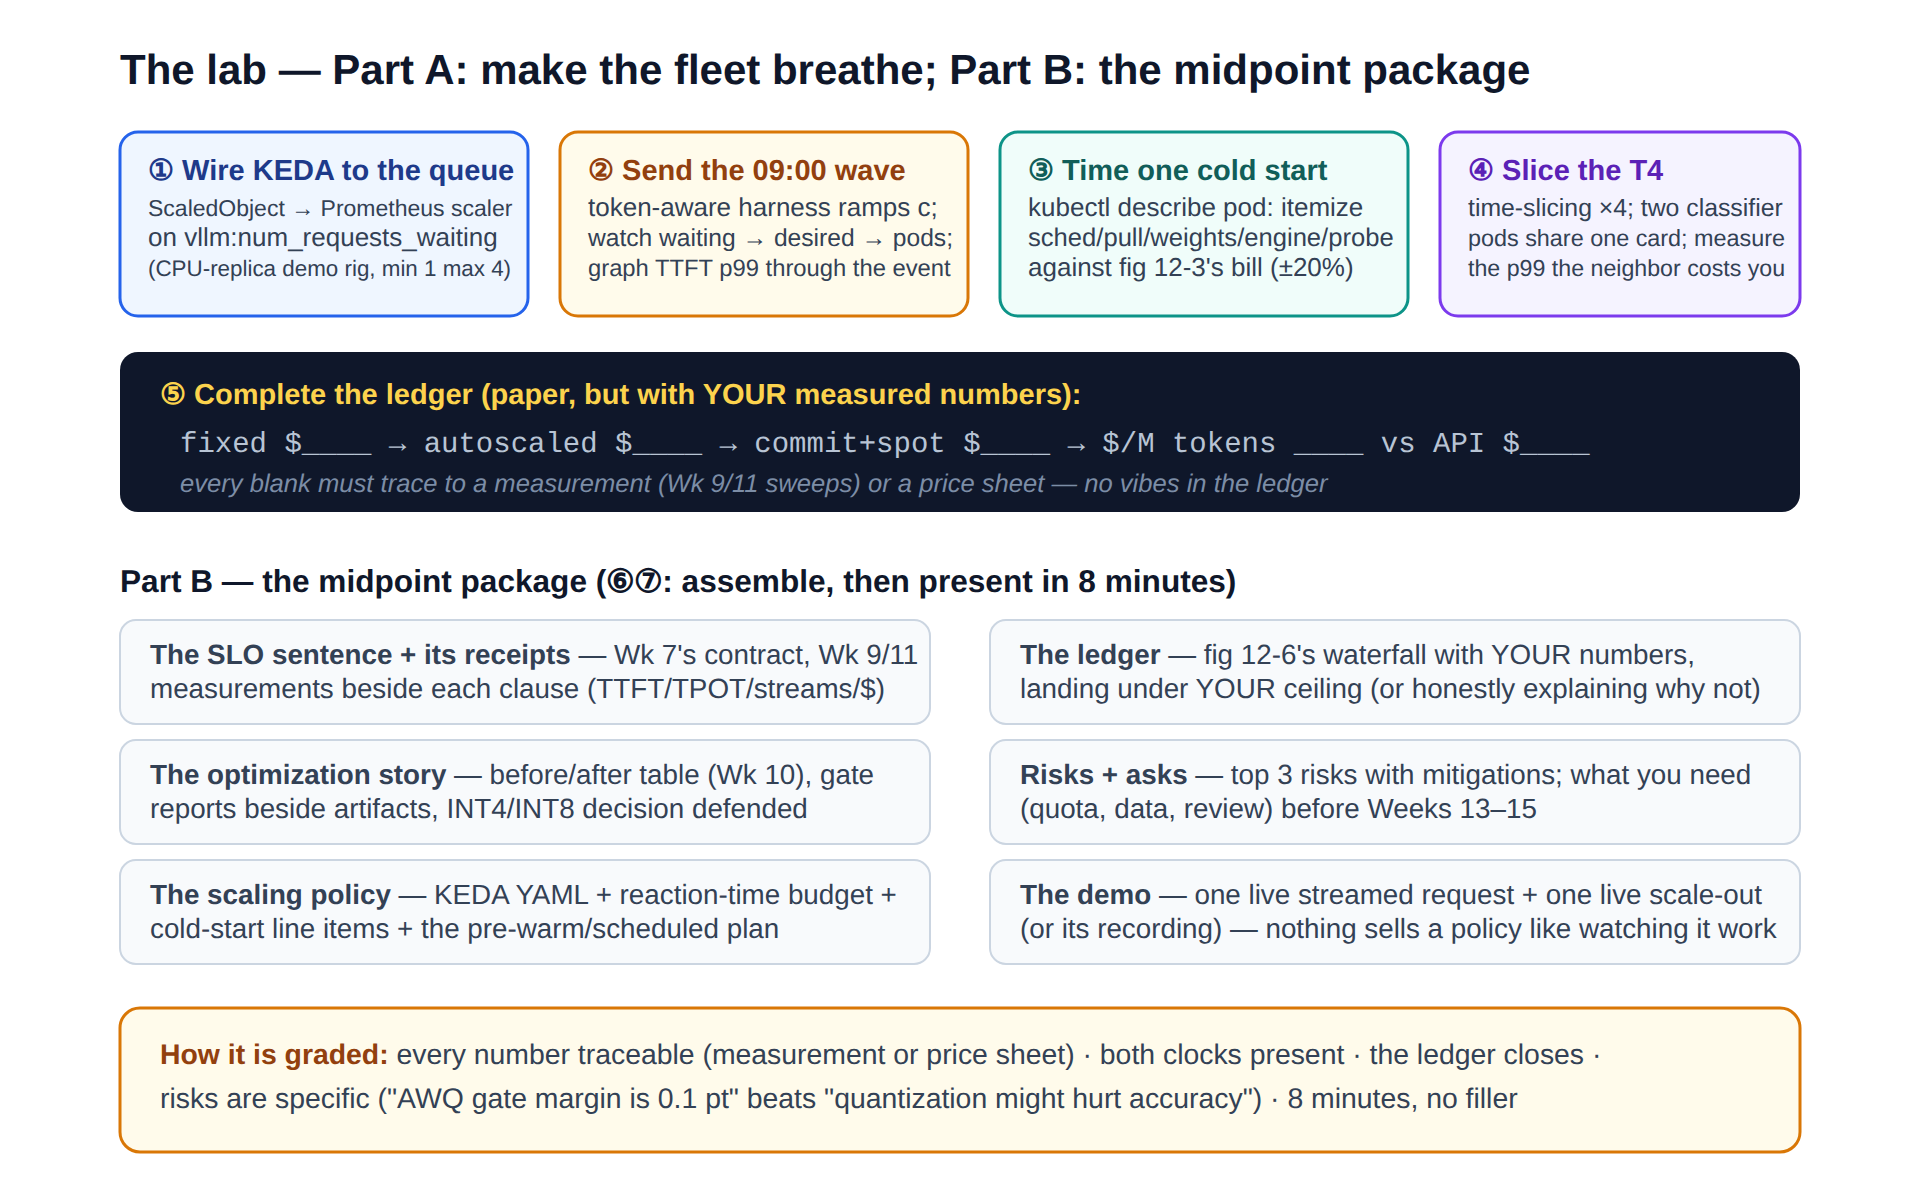
\includegraphics{figures/fig12-7_midpoint.png}}\\[3pt]
  \figcaption{그림 12-7  실습의 두 부분. A에서는 스케일러를 연결하고 파도를 보내며 탄생 시간을 재고 T4를 분할해 네 가지를 측정한다. B는 모든 수치의 출처를 추적할 수 있는 산출물 여섯 개로 구성한 8분짜리 중간 점검 패키지다.}
\end{tbbfigure}

\subsection*{A부 — 네 가지 측정(①–⑤)}

\begin{tbbitemize}
  \item \textbf{① KEDA를 대기열에 연결한다.} 실습 자료의 데모 환경을 배포한다. GPU 네 대 없이도 스케일링이 보이도록 CPU 모드 레플리카를 사용한다. Prometheus + KEDA + 기록 12-1의 ScaledObject를 \code{vllm:num\_requests\_waiting}에 연결하고 최소 1 / 최대 4로 설정한다. KEDA가 생성한 HPA 객체를 확인한다. 한 단계 위에서 관리자를 관리하는 제5장의 패턴이다.
  \item \textbf{② 09:00 파도를 보낸다.} 제11장의 토큰 인식 하네스로 동시성을 높이고 세 터미널(\code{kubectl get hpa -w}, \code{get pods -w}, 하네스의 TTFT 로그)에서 \code{waiting → desired → pods}를 지켜본다. 사건 전체의 TTFT p99 그래프를 그리고 감지, 탄생, 드레인을 표시한다. 이어 08:40 cron 트리거를 추가하고 같은 파도를 보낸다. GPU 비용 \textasciitilde{}\$0로 그래프 두 개와 교훈 하나를 얻는다.
  \item \textbf{③ 실제 탄생 하나의 시간을 잰다.} GPU 노드에서 vLLM 포드를 삭제하고 \code{kubectl describe pod} + 엔진 로그를 사용해 기록 12-3의 항목을 초시계로 잰다. 각 줄을 담당 장과 ±20\% 안에서 맞추고 플릿의 지배 항목과 이를 공격할 사다리 단을 제시한다. 이 수치는 \textit{자신의} 반응 시간 예산으로 중간 점검 패키지에 들어간다.
  \item \textbf{④ T4를 분할하고 대가를 측정한다.} 시분할 ConfigMap(replicas: 4)을 적용하고 분류기 포드 두 개를 함께 스케줄링한 뒤, 9주 차 스윕을 단독 대 이웃 있음으로 다시 실행한다(기록 12-4). 두 경우의 p50, p99, req/s@SLO를 보고하고 SLO 아래에서 시분할에 관한 한 문장 결론을 작성한다.
  \item \textbf{⑤ 원장을 마감한다.} 기록 12-6의 빈칸을 \textit{자신이} 측정한 수치로 채운다. 실제 하루의 지표나 실습 자료 재생에서 얻은 계단, rep-h/day, 실시간 가격표에서 정한 포트폴리오 분할, API 대안과 비교한 \$/M tokens를 넣는다. 모든 빈칸의 출처를 측정값이나 가격표로 추적할 수 있어야 한다. 채점자가 가장 먼저 확인하는 항목이다.
\end{tbbitemize}

\subsection*{B부 — 중간 점검 패키지(⑥–⑦)}

산출물 여섯 개를 조립한 뒤 8분에 맞춰 연습한다. \textbf{근거가 있는 SLO 문장}은 7주 차 계약을 11주 차 조항으로 다시 쓰고 각 조항 옆에 이를 인증하는 측정값을 둔다. \textbf{최적화 이야기}에는 10주 차 전후 표, 산출물 옆의 게이트 보고서, 한 문단으로 옹호한 INT4/INT8 결정을 넣는다. \textbf{스케일링 정책}은 ScaledObject, ③의 반응 시간 예산, cron/사전 워밍업 계획, 파도를 견딘 모습을 보여 주는 ②의 그래프 하나로 구성한다. \textbf{원장}은 자신의 수치를 넣은 그림 12-6의 폭포이며 상한 아래에 도달하거나 격차와 계획을 정직하게 설명한다. \textbf{위험과 요청 사항}에는 완화책이 있는 구체적인 위험 세 가지와 13–15주 차 전에 필요한 것을 넣는다. "안전 슬라이스에서 AWQ 게이트 여유가 0.1 pt다"가 "양자화가 정확도를 해칠 수 있다"보다 낫다. \textbf{데모}에서는 스트리밍 요청 하나와 실시간 스케일 아웃 하나 또는 녹화를 보여 준다. 발표하고 피드백을 수집한다. 15주 차의 드레스 리허설이다.

\begin{calloutbox}{tbbteal}{tbbxF0FDFA}
{\normalsize\bfseries\color{tbbx115E59}상자 12-2  중간 점검 평가 기준 — 8분을 채점하는 방법}\par\vspace{3pt}
\begin{tbbitemize}
  \item \textbf{추적 가능성(40\%)} — 모든 수치가 스윕, 기록, 가격표를 인용해야 한다. 출처 없는 "약 500"은 이 교재에서 유일하게 실패하는 답이다.
  \item \textbf{두 시계 제시(20\%)} — 백분위수와 부하를 명시한 TTFT와 TPOT를 모두 보여 준다. "지연 시간" 하나만 쓰면 해당 행 점수를 잃는다. 상자 11-2의 규칙은 계속 살아 있다.
  \item \textbf{원장 마감(20\%)} — 고정 → 오토스케일링 → 포트폴리오 → 단위 비용의 계산을 실시간으로 확인할 수 있어야 한다. 상한 아래라고 추가 점수를 주지 않고, \textit{설명하지 않은} 격차는 감점한다.
  \item \textbf{위험을 엔지니어링으로 표현(10\%)} — 구체적이고 측정했으며 완화해야 한다. 하나 이상은 약정 대 로드맵, 스팟 가용성, 이그레스 같은 비용 위험이어야 한다.
  \item \textbf{시간 규율(10\%)} — 8분 발표 후 질문을 받는다. 말을 멈추지 못하는 스태프 엔지니어는 용량 검토 일정이 다시 잡히며 학생도 마찬가지다.
\end{tbbitemize}
\end{calloutbox}

\vspace{3.0pt}

제출물은 A부의 측정 산출물 네 개(파도 그래프 두 개, 항목별 탄생, 이웃 세금 표), 완성한 원장, 슬라이드나 문서 형태의 산출물 여섯 개 패키지, 그리고 이 교재에서 기술 실습으로는 마지막인 결제 내역 스크린샷이다. 이 장을 마치면 스크린샷은 더 이상 의례가 아니라 \textbf{읽을 수 있는 명세}가 된다. 모든 항목에 담당 장, 수단, 소유자가 생겼다. 처음부터 바로 그것이 목적이었다.

\begin{calloutbox}{tbbpurple}{tbbpurplefill}
{\normalsize\bfseries\color{tbbpurple}생각해 보기}\par\vspace{3pt}
\begin{tbbitemize}
  \item ②의 그래프에서 cron 실행은 +\$1.07/day의 비용으로 TTFT p99를 0.46 s에 평평하게 유지하지만 반응형 실행은 추가 비용 없이 3 min 동안 위반한다. 자신의 제품을 위한 두 문장 권장안을 작성하고, 결정을 좌우하는 인프라 사실이 아닌 제품 사실을 제시하라.
  \item ③에서 탄생은 150초가 아니라 190 s였다. 추가 40 s는 노드 캐시가 없는 새 노드의 첫 포드가 이미지를 풀하는 시간이다. 어느 사다리 단으로 해결할 수 있고 각각의 월 비용은 얼마인가? 플릿이 주 2회 노드를 교체한다면 실제로 무엇을 권장할지 설명하라.
  \item 중간 점검 검토자가 "원장은 일중 곡선이 유지된다고 가정한다. B2B 고객이 02:00에 50k requests의 야간 배치를 추가하면 무엇이 깨지는가?"라고 묻는다. 계단과 포트폴리오에서 어느 계층이 처리하는지, 부하율에 미치는 영향으로 답하라. 이것이 단위 비용에는 좋은 소식인 이유도 설명하라.
  \item 팀의 위험 세 줄을 초안으로 지금 작성하라. 9/11주 차 측정에서 SLO 위험 하나, 이 장의 원장에서 비용 위험 하나, 13–15주 차의 전달 위험 하나를 택한다. 평가 기준의 구체성 잣대를 자신의 문장에 적용해 한 번 수정하라.
\end{tbbitemize}
\end{calloutbox}

\namedsection{요약}{열여섯 가지 핵심 내용}

\qitem{1}{\textbf{낭비는 잘못된 설정이 아니라 구조에서 나온다.} 수요는 시간에 따라 모양이 있지만 정적 플릿은 수평선이다. 측정한 사례 12-A에서는 하루 61레플리카 시간이 필요하지만 96시간에 비용을 냈다. 부하율은 63.5\%, 야간 근무 비용은 \$868/month다. 사례 1-B의 유령 GPU를 일중 곡선으로 확장한 모습이다.}

\qitem{2}{\textbf{1902년의 문제를 1910년까지 해결했다.} Samuel Insull은 부하율(평균 ÷ 피크)로 시카고 전력망을 운영했다. 수요를 계량하고 고객 피크를 맞물리게 하며 골짜기를 저렴하게 팔고 피크에는 중단 가능한 부하를 끊었다. 이 장의 오토스케일링, 공유, 스팟, 야간 배치는 모두 그의 기법이다.}

\qitem{3}{\textbf{오토스케일러는 기상학자가 아니라 온도 조절기다.} 15 s마다 desired = ceil(current × metric ÷ target)을 계산해 제5장의 메커니즘이 따르는 정수 하나에 쓴다. 엔지니어링은 공식이 아니라 지표와 초시계에 있다.}

\qitem{4}{\textbf{공급 게이지가 아니라 수요 신호로 스케일링한다.} GPU가 빠지는 동안 CPU는 9\%라 CPU\%는 GPU 서비스에서 작동하지 않는다. 제9장 사례의 거울상이다. GPU 사용률은 포화되고 부분 부하에서 거짓말한다. 올바른 눈은 선행하고 상한이 없으며 사용자가 느끼는 입장 대기열(vllm:num\_requests\_waiting)이다(L = λW).}

\qitem{5}{\textbf{루프의 성향은 비대칭이어야 한다.} 순간 신호로 증가시키고 후행 창에서만 감소시킨다(안정화/쿨다운 \textasciitilde{}300 s). 손실 함수가 비대칭이기 때문이다. 빠른 증가는 레플리카 몇 분을 낭비하지만 빠른 감소는 SLO를 깨뜨린다. 플래핑은 청구서를 제10장의 torch.compile 악순환 같은 콜드 스타트 오버헤드로 바꾼다.}

\qitem{6}{\textbf{반응 시간도 용량의 일부다.} T = 감지(≤15 s) + 결정(≤15 s) + 탄생(따뜻한 노드 \textasciitilde{}150 s)이다. 대기열은 T 전체에 걸쳐 초과분을 적분한다. 반응형 경로에서 09:00 파도는 3분 동안 TTFT를 위반하지만, 08:40 cron은 \$1.07로 없앤다. 볼 수 있는 피크에는 예지력보다 달력이 낫다.}

\qitem{7}{\textbf{포드는 파도를 쫓고 노드는 예측을 따른다.} GPU 노드 탄생은 3–7 min이고 때로는 "no capacity"로 끝난다. SLO 경로에 두지 않는다. 하루의 노드 범위를 미리 프로비저닝하고 그 안에서 포드를 오토스케일링한다.}

\qitem{8}{\textbf{콜드 스타트는 항목별 청구서다.} 스케줄링 2 s + 이미지 16 s(제4장) + 가중치 9 s(제6장) + 엔진 초기화 95 s(제11장) + 워밍업 28 s(제5/10장) = 150 s다. Firecracker의 125 ms는 환경 항목을 해결했고 페이로드 항목은 사용자의 몫이다. 서버리스 GPU는 프리미엄을 내고 따뜻한 풀 + 초기화한 프로세스의 스냅샷/복원을 사용하는 것이다.}

\qitem{9}{\textbf{완화 사다리는 이미 배운 장으로 이루어진다.} 작고 캐시되며 지연 로드하는 이미지 → 병렬 가중치 가져오기 + 노드 캐시 → 준비 상태 안의 워밍업 → 여유 용량 +1 (\textasciitilde{}\$50/mo) → 예약 스케일링 → 0으로 스케일링 순이다. 0은 호출자가 첫 적중의 몇 분 지연을 감당하는 엔드포인트용이다. 롱테일은 잠들고 SLO를 지는 헤드는 롤아웃과 03:00 사용자를 위해 바닥 2개를 유지한다.}

\qitem{10}{\textbf{공유는 카드당 테넌트 하나 규칙을 세 방식으로 굽힌다.} 시분할은 전체 다이를 번갈아 쓰며 격리가 없어 개발용으로만 적합하다. 실습에서 이웃 하나로 p99가 9.8 → 38.4 ms가 되었다. MPS는 동시에 실행하지만 장애 반경이 하나라 한 팀의 작은 모델에 적합하다. MIG는 큰 다이를 최대 7개로 하드웨어 분할해 자체 SM/L2/DRAM/OOM을 제공하므로 SLO가 있는 멀티테넌트에 안전하지만 T4/L4에는 없다.}

\qitem{11}{\textbf{통합 계산은 Insull의 다양성 기법이다.} A100의 1g.10gb 조각(≈\$0.51/hr)은 조각 여섯 개를 남기면서 T4 전체(\$0.53)와 비슷하다. 단, 테넌트 피크가 맞물리고 조각이 자체 §10.2 진단을 통과해야 한다. 대역폭도 1/7이다. 상관된 피크는 한 계층 아래에서 13:00 문제를 다시 만든다.}

\qitem{12}{\textbf{KServe는 제9장이 이름 붙인 플랫폼 종이다.} 15줄 InferenceService 하나가 Deployment, 프로브, 모델 가져오기, 런타임, 인그레스(ingress), 동시성 기반 오토스케일러, 0으로 스케일링, 카나리 트래픽 분할을 만든다. 모델과 팀이 늘면 도입하고 인기 모델 하나가 제품이면 원시 Deployment + KEDA를 유지한다.}

\qitem{13}{\textbf{용량을 포트폴리오로 구매한다.} 바닥은 약정(−30–60\%), 어깨는 온디맨드, 버스트는 스팟(−60–90\%, 30 s–2 min 통보), 골짜기는 배치로 채운다. 바닥을 스팟에 두지 않는다. 드레인 훈련은 제5장의 preStop + 제11장의 상태 비저장이다. 스트림을 끝내고 등록을 해제한 뒤 다른 곳에서 다시 프리필한다. 짧은 지연일 뿐 잘못된 답은 아니다.}

\qitem{14}{\textbf{원장을 상한 아래에서 마감했다.} \$4,762(7주 차 추정) → \$2,381(10주 차 INT8) → \$1,513(오토스케일링, 61 rep-h/day) → \textbf{\$877}(= \$714 약정 + \$113 스팟 + \$50 사전 워밍업) < \$900이다. 모든 단계가 \textit{같은} SLO에서 측정한 수단이다.}

\qitem{15}{\textbf{단위 경제성이 제1장의 손익분기점을 마무리한다.} \$877 ÷ 서빙한 2.0B tokens = \$0.44/M으로 API의 \$0.50보다 낮다. 자체 호스팅은 \textit{이} 사용률에서 이기지만 절반이면 진다. 자체 구축 대 외부 도입은 구호가 아니라 부하율 문제였다.}

\qitem{16}{\textbf{FinOps는 감시하는 용량이다.} 총액이 아니라 \$/M tokens를 계량하고, 태그와 비용 공개로 NAT 함정이 태그 없는 배관에 숨지 않게 하며, 예측의 80/100/120\%에서 이상 경보를 건다. 중간 점검 패키지는 모든 수치의 출처를 추적할 수 있게 8분에 이를 발표한다. 15주 차의 드레스 리허설이다.}

\namedsection{연습문제}{}

\subsection*{A. 객관식}

\qitem{1}{GPU 채팅 서비스가 대기열 증가와 붉은 TTFT로 고전하지만 CPU 기반 HPA는 전혀 스케일링하지 않는다. 근본 원인은 무엇인가?}

\begin{tbboptions}
  \item ① HPA 루프가 너무 느리다        ② 경합 자원인 GPU/대기열이 관찰 지표에 보이지 않는다. CPU는 9\%로 쉰다
  \item ③ maxReplicas가 너무 낮다        ④ 이미지가 너무 크다
\end{tbboptions}

\qitem{2}{vLLM 플릿의 최적 오토스케일링 지표가 num\_requests\_waiting인 이유는 무엇인가?}

\begin{tbboptions}
  \item ① 수집 비용이 가장 저렴하다        ② 지연 시간이 움직이기 전 작동하는 선행 지표이고, 용량 오차의 크기를 나타내는 상한 없는 값이며, TTFT의 분자인 대기열로 사용자가 느낀다
  \item ③ Kubernetes에 내장되어 있다        ④ 정상 상태에서 언제나 0이다
\end{tbboptions}

\qitem{3}{스케일 업 창은 즉시 반응하지만 스케일 다운 창은 \textasciitilde{}5분인 이유는 무엇인가?}

\begin{tbboptions}
  \item ① 스케일 다운이 기계적으로 더 느리다        ② 손실 함수가 비대칭이다. 빠른 증가는 레플리카 몇 분을 낭비하지만 빠른 감소는 SLO를 깨뜨리고 콜드 스타트 비용을 다시 내며 플래핑한다
  \item ③ Kubernetes가 요구한다        ④ 5분 단위로 요금을 부과한다
\end{tbboptions}

\qitem{4}{레플리카 2개, 전체 대기 41개, 레플리카당 목표 10일 때 HPA가 계산하는 desired는 얼마인가?}

\begin{tbboptions}
  \item ① 3        ② 4        ③ ceil(2 × 20.5 ÷ 10) = 5 (이후 maxReplicas로 제한)        ④ 41 ÷ 10 = 4.1 → 4
\end{tbboptions}

\qitem{5}{Firecracker의 125 ms microVM이 GPU 콜드 스타트를 해결하지 못한 이유는 무엇인가?}

\begin{tbboptions}
  \item ① CPU에서만 실행된다        ② 청구서의 대부분이 환경이 아니라 페이로드다. 수 기가바이트의 이미지와 가중치, CUDA 컨텍스트, 엔진 초기화가 150초 중 148초를 차지한다
  \item ③ Kubernetes는 microVM을 사용할 수 없다        ④ GPU는 부팅이 느리다
\end{tbboptions}

\qitem{6}{0으로 스케일링이 적합한 대상은 무엇인가?}

\begin{tbboptions}
  \item ① 유휴 시간이 있는 모든 서비스        ② 야간의 채팅 플릿
  \item ③ 호출자가 첫 적중의 몇 분 지연을 감당할 수 있는 엔드포인트. 롱테일 내부 모델, 개발 엔드포인트, 배치 트리거 스코어러        ④ GPU에서는 아무것도 해당하지 않는다
\end{tbboptions}

\qitem{7}{한 팀이 SLO를 지는 서비스 두 개를 시분할 GPU 한 대에 둔다. 예상되는 결과는 무엇인가?}

\begin{tbboptions}
  \item ① 처리량 2×        ② 아무것도 변하지 않는다
  \item ③ p50은 거의 유지되지만 운 나쁜 요청이 이웃의 시간 조각을 먹어 p99가 몇 배가 된다. 테넌트 하나의 OOM이 둘 다 죽인다        ④ MIG가 자동 활성화된다
\end{tbboptions}

\qitem{8}{일중 계단의 포트폴리오 규칙은 무엇인가?}

\begin{tbboptions}
  \item ① 할인을 위해 모두 스팟에 둔다        ② 할인을 위해 모두 약정한다
  \item ③ 바닥은 약정하고 어깨는 온디맨드, 버스트는 스팟으로 처리하며 바닥을 스팟에 두지 않는다        ④ 온디맨드만 쓴다. 가격 전략은 엔지니어링이 아니다
\end{tbboptions}

\subsection*{B. 단답형}

\qitem{1}{GPU 플릿의 부하율을 정의하고 사례 12-A(필요 61, 결제 96)에서 계산한 뒤, 이 지표로 전력 회사를 운영한 1900년대 인물을 제시하라.}

\qitem{2}{목표 레플리카 공식을 쓰고 다음 조건에서 계산하라. 레플리카 3개, 전체 대기 66개, 레플리카당 목표 15, maxReplicas 6이다.}

\qitem{3}{따뜻한 노드의 150초 콜드 스타트를 담당 장과 함께 다섯 항목으로 세분화하고, vLLM 플릿에서 지배적인 항목을 밝히라.}

\qitem{4}{시분할, MPS, MIG를 각각 무엇을 격리하거나 격리하지 않는지 중심으로 한 문장씩 설명하라.}

\qitem{5}{스팟 드레인 훈련의 네 박자를 서술하고, 중단된 스트림이 잘못된 답이 아니라 짧은 지연만 겪게 하는 제11장의 성질을 제시하라.}

\qitem{6}{중간 점검 원장은 왜 월 지출 대신 \$/M tokens를 보고하는가? 비교 가능성과 제1장의 어느 질문에 답하는지를 모두 설명하라.}

\subsection*{C. 서술형}

\qitem{1}{용량 검토에 관한 글을 작성하라. 서비스는 평일 11:00–15:00에 동시 스트림 340개로 피크를 찍고, 어깨는 120개, 야간과 주말 바닥은 25개다. 레플리카당 좌석 32개, \$1.10/hr, 콜드 스타트 3 min이다. 계단, 반응 계획(cron + 대기열 트리거 + 여유 용량), 포트폴리오(1년 약정 −38\%, 스팟 −64\%를 사용하는 약정/온디맨드/스팟), 최종 월 청구서를 구성하라. Insull 방식으로 전후 부하율도 제시하라.}

\qitem{2}{"오토스케일링은 이 장에서 가장 덜 흥미로운 수단이다. 실제 비용 절감은 제10장과 제11장에서 일어났고 실제 위험은 여기 있다"라는 주장을 옹호하거나 공격하라. 교재 원장(\$4,762 → \$2,381 → \$1,513 → \$877), 각 수단이 만드는 SLO 위반 유형, 각 단계의 엔지니어링 비용을 활용하라. 이 프로젝트에서 엔지니어링 비용의 다음 한계 달러를 어디에 써야 하는가?}

\qitem{3}{통합에 관한 글을 작성하라. 한 부서가 작은 모델 아홉 개를 각각 T4 한 대(\textasciitilde{}\$0.53/hr, 사용 주기 5–40\%, 팀 세 개, SLO를 지는 모델 두 개)에서 실행한다. 시분할/MPS/MIG/전체 카드로 목표 플릿을 설계하라. 모델 클래스별 배치, 각 선택의 격리 논거, 장애 반경과 재구성 드레인 위험, 월 전후 비용을 포함하라. 승인 전에 요구할 측정 하나도 제시하라. 힌트는 Insull의 요구다.}

\qitem{4}{손익분기점에 관한 글을 작성하라. 최종 원장(\$877, 서빙한 2.0B tokens, 용량 3.1B)을 사용해 월 토큰의 함수로 자체 호스팅 대 API 결정을 도출한다. \$0.50/M API와의 교차점을 계산하고 INT4 (1.6×)와 트래픽 두 배가 각각 이를 어떻게 움직이는지 보인 뒤, 0.4B tokens/month인 스타트업에 보내는 한 문단 메모로 마무리하라.}

\namedsection{정답과 해설}{}

\subsection*{A. 객관식}

\qitem{1}{\textbf{②} 오토스케일러의 눈이 경합하지 않는 자원을 본다. 제9장 사례 A의 거울상이다. 그때는 CPU가 고정되고 GPU가 쉬었지만 여기서는 GPU가 고전하는 동안 CPU가 쉰다. 수요 신호로 스케일링해야 한다. (§12.2)}

\qitem{2}{\textbf{②} 한 지표가 세 속성을 모두 갖고 있으며 제11장에서 읽는 법을 배우고 기록 11-3에서 관찰한 바로 그 항목이다. 공급 게이지인 CPU\%, GPU\%는 세 속성 중 하나 이상에서 실패한다. (§12.2)}

\qitem{3}{\textbf{②} 비대칭은 레플리카 몇 분과 SLO 위반 + 다시 내는 탄생 비용을 비교하는 손실 함수를 인코딩한다. 플래핑의 최악 사례는 제10장의 스케일 아웃 시 컴파일 생각해 볼 문제다. (§12.2)}

\qitem{4}{\textbf{③} 레플리카당 지표는 20.5다. desired = ceil(2 × 20.5/10) = ceil(4.1) = 5를 계산한 뒤 상한을 적용한다. ④는 고전적 오류다. 공식은 현재 수를 스케일링하며 원시 합계를 나누는 것이 아니다. (§12.2)}

\qitem{5}{\textbf{②} 기록 12-3에서 환경은 150초 중 \textasciitilde{}2 s만 차지한다. Firecracker는 2005년 문제를 훌륭하게 해결했지만 2026년 문제는 수 기가바이트와 CUDA 컨텍스트다. 더 빠른 부팅이 아니라 따뜻한 풀과 스냅샷이 필요하다. (§12.3)}

\qitem{6}{\textbf{③} 결정 규칙은 유휴 시간이 아니라 호출자의 지연 시간 허용 범위다. (a)는 이를 충족하지 못한다. 03:00 사용자도 실제이고 바닥은 롤아웃에도 필요하다. (§12.3)}

\qitem{7}{\textbf{③} 기록 12-4의 측정값은 p50 3.1 ms, p99 38.4 ms다. 꼬리 요청이 컨텍스트 전환과 이웃의 배치를 먹으며 VRAM은 공유한다. SLO 아래의 시분할은 제14장의 전쟁 이야기를 미리 구매하는 셈이다. (§12.4)}

\qitem{8}{\textbf{③} 계단은 계층별로 요금표에 대응한다. 바닥을 스팟에 두는 것은 점검표에서 가장 붉은 위험 신호다. 03:00에 회수되면 대체 용량이 없다. (§12.5)}

\subsection*{B. 단답형}

\qitem{1}{부하율 = 필요한(또는 평균) 용량 시간 ÷ 결제한(또는 피크) 용량 시간이다. 61/96 = \textbf{63.5\%}다. Chicago Edison의 Samuel Insull은 수요 곡선으로 전력 가격을 정하고 골짜기를 채워 바로 이 수치를 높였다. (§12.1)}

\qitem{2}{desired = ceil(current × metric ÷ target) = ceil(3 × 22 ÷ 15) = ceil(4.4) = \textbf{5}다. 상한 6 이하여서 5가 유지된다. 레플리카당 지표는 66/3 = 22다. (§12.2)}

\qitem{3}{스케줄링 2 s(제5장) + 이미지 풀 16 s(제4장) + 가중치 9 s(제6장) + \textbf{엔진 초기화 95 s(제11장 — VRAM 로드, KV 풀, CUDA 그래프. 지배 항목)} + 프로브 워밍업 28 s(제5/10장) = 150 s다. (§12.3)}

\qitem{4}{시분할은 테넌트가 전체 다이를 번갈아 써 아무것도 격리하지 않는다. MPS는 SM 상한을 두고 동시에 실행해 연산 몫은 격리하지만 대역폭과 장애는 격리하지 않는다. MIG는 자체 SM/L2/DRAM/OOM을 지닌 하드웨어 파티션으로 거의 모든 것을 격리하지만 큰 다이에서만 1/7 세분성을 제공한다. (§12.4)}

\qitem{5}{통보 → 새 입장 중단(준비 상태 해제) → 유예 기간 안에 진행 중 스트림 완료 → 등록 해제 순이다. 각 요청에 전체 기록을 담고 KV가 계약이 아닌 캐시인 상태 비저장 덕분에 회수된 스트림은 다른 곳에서 다시 프리필한다. 짧은 지연이 있지만 답은 정확하다. (§12.5, 제5/11장)}

\qitem{6}{단위 비용은 주, 모델, 플릿 크기, API의 공개 \$/M과 비교할 수 있지만 총지출은 성장만 측정한다. 또한 이 사용률에서 \$0.44 대 \$0.50이라는 제1장의 자체 구축 대 외부 도입 질문에 직접 답한다. (§12.5)}

\subsection*{C. 서술형(채점 기준)}

\qitem{1}{계단은 피크 ceil(340/32)=11 (4 h), 어깨 ceil(120/32)=4 (평일 \textasciitilde{}8 h), 바닥 ceil(25/32)=1→\textbf{2}(운영 바닥)이므로 평일 \textasciitilde{}76 rep-h, 주말 \textasciitilde{}48이다. 반응 계획은 3분 탄생을 고려해 10:40에 cron으로 11개까지 늘리고, 형태에는 대기열 트리거를 쓰며, 11:00–15:00에 여유 용량 +1을 둔다. 포트폴리오는 2개 약정(−38\%), 어깨 온디맨드, 7레플리카 버스트 스팟(−64\%)이다. 좋은 답은 고정 11×24 = 264 rep-h/day와 평균 \textasciitilde{}72를 비교해 부하율 \textasciitilde{}27\% → 이후 \textasciitilde{}64\%에 가까운 계산을 보인다. 일관된 청구서는 인정하지만 바닥을 스팟에 두거나 파도 안에 노드 탄생을 두면 감점한다. (§§12.1–12.5)}

\qitem{2}{좋은 글은 "흥미로움"과 "가치"를 구분한다. 오토스케일링 절감은 \$868/mo이며 2,381→1,513이 스케일러, 1,513→877이 포트폴리오다. 제10장의 \$2,381 절감이 더 컸다. 하지만 오토스케일링은 플래핑, 콜드 스타트 매복, 잘못된 지표로 위반을 \textit{만들 수 있는} 고유한 위험이 있어 엔지니어링의 대부분은 안전에 관한 것이다. 다음 한계 비용은 이 프로젝트에서 §12.3의 95 s 엔진 초기화나 원장의 서빙/용량 격차에 투입할 가능성이 크다. 후자는 인프라가 아니라 마케팅 문제다. 수단이 곱셈으로 합성되고 SLO 위반 인용 규율(상자 12-1)이 실제 논지임을 알아보는 글을 높이 평가한다. (장 전체)}

\qitem{3}{포함할 내용: SLO를 지는 두 모델은 MIG 조각에 두되 피크가 상관되면 전체 카드를 고려한다. 한 팀의 작은 모델 묶음은 MPS, 개발/노트북은 시분할, 카드를 채우는 모델은 전체 카드를 쓴다. 위험은 노드 수준 장애 반경(두 SLO 모델을 안티어피니티로 분산), MIG 재구성 드레인(노드 풀별 프로파일), 조각 대역폭과 모델별 §10.2 진단이다. 요구할 측정은 \textbf{아홉 사용 주기의 피크 상관관계}, 즉 Insull의 다양성이다. 상관된 피크를 통합하면 문제를 재현한다. 다양성이 있을 때만 전후가 약 9 × \$394 → A100 한 대(\textasciitilde{}\$2,678) + 전체 카드 1–2대가 된다. (§12.4)}

\qitem{4}{자체 호스팅 비용은 대략 고정 바닥 + 가변 rep-h다. 바닥 위에서는 토큰에 거의 선형이고 아래에서는 평평하므로 규모가 늘수록 단위 비용이 떨어진다. Insull의 원리다. 교재 수치로 \$0.50/M과 교차하는 지점은 \textasciitilde{}1.7–1.8B tokens/mo다. 아래는 바닥이 지배하고 위는 포트폴리오 가격이 지배한다. INT4는 rep-h당 토큰을 늘려 교차점을 \textasciitilde{}1.6× 낮추고, 트래픽 두 배는 같은 플릿을 활용해 \$0.28/M로 낮춘다. 0.4B/mo에서는 API가 \textasciitilde{}2× 유리하다. 메모에는 "지금은 구매하고 \textasciitilde{}1.5B/mo 또는 데이터 거버넌스가 자체 호스팅을 강제할 때 다시 검토"라고 쓰며 지배 입력인 사용률과 tokens/replica를 인용한다. 일관된 계산은 인정하고 구호는 인정하지 않는다. (§12.5, 제1장 §1.5)}

\namedsection{더 읽을거리}{}

\textbf{[이번 주]}로 표시한 자료는 실습을 직접 뒷받침하고, \textbf{[N주 차]}는 나중에 도움이 될 자료를 뜻한다.

\begin{tbbitemize}
  \item \textbf{[이번 주] Kubernetes HPA documentation — "Horizontal Pod Autoscaling" (algorithm + behavior/stabilization)} 및 \textbf{KEDA docs — ScaledObject, Prometheus scaler, cron scaler} — 기록 12-1/12-2의 권위 있는 출처다. behavior 절은 §12.2의 성향을 그대로 설명한다.
  \item \textbf{[이번 주] NVIDIA MIG User Guide · GPU Operator time-slicing docs} — 제2장 §2.6이 이번 주 직접 다룬다고 약속한 프로파일, K8s 장치 플러그인 전략, 재구성 드레인 주의점을 운영 관점에서 설명한다.
  \item \textbf{[이번 주] KServe documentation — InferenceService \& autoscaling} — 제9장의 "CRD를 훑고 12주 차에 배포하라"는 과제를 수행할 때가 되었다. 동시성 기반 기본값은 §12.2가 제도화된 모습이다.
  \item \textbf{A. Agache et al., "Firecracker" (NSDI 2020), §§1–2 다시 읽기} — 2주 차 필독 자료를 두 번째로 읽는다. 이번에는 "내 150초 중 무엇을 해결하는가?"라고 물어보자. 답이 "2초"라는 사실이 §12.3의 교훈이다.
  \item \textbf{클라우드 공급자 문서: Spot best practices (AWS) / Preemptible \& Spot VMs (GCP) · committed-use discounts / Savings Plans} — 통보 창, 용량 최적화 할당, 약정 범위 등 포트폴리오의 작은 글씨다. §12.5 형태의 계약에 서명하기 전에 읽어야 한다.
  \item \textbf{J. F. Wasik, "The Merchant of Power" (2006)} — Insull의 전기로 부하율, 수요 계량기, 맞물리는 피크, 전력 경제학의 탄생을 다룬다. 이 장의 중심 이야기를 책 한 권으로 확장하며 이 장에서 생략한 경고성 결말도 있다.
  \item \textbf{"Sub-second GPU cold start" 계열 엔지니어링 글(Modal, Fly.io, Cloud Run GPU) + containerd 지연 풀(eStargz) 문서} — 제4장이 콜드 스타트 최전선으로 예고한 스냅샷/복원, 이미지 스트리밍, 따뜻한 풀 경제성을 다룬다.
  \item \textbf{[이번 주, 재미] 내림차순으로 정렬한 클라우드 콘솔 결제 페이지} — NAT gateway(제6장), 유휴 개발 GPU, 태그 없는 수수께끼를 찾아보자. 이 장을 마치면 의례가 아니라 명세처럼 읽힌다. 모든 줄에 수단과 소유자가 있다.
\end{tbbitemize}

\vspace{5.0pt}

\begin{calloutbox}{tbbblue}{tbbbluefill}
{\normalsize\bfseries\color{tbbblue}다음 장 — 제13장: MLOps와 배포 자동화}\par\vspace{3pt}
플릿은 이제 숨 쉬고 원장도 마감되었다. 하지만 이 교재에서 배포한 모든 개선은 \textbf{사람이 kubectl을 입력해} 배포했다. 기록 12-5에는 \code{canaryTrafficPercent: 10}이라는 조절점이 매달린 채 남았다. 아무도 제어하지 않는 트래픽 분할이다. 제13장은 그 운전자를 만든다. 제4장의 다이제스트와 제6장의 저장소를 승격 워크플로로 발전시킨 \textbf{모델 레지스트리와 버전 관리}, 모든 후보에 제10장의 게이트와 제9장의 스윕을 실행하는 \textbf{CI/CD 파이프라인}(실습에서는 GitHub Actions), 오프라인 게이트가 확인할 수 없는 것을 10\% 분할로 검사하는 \textbf{카나리, A/B, 섀도 배포(shadow deployment)}, 그리고 오퍼레이터까지 외주화한 KServe와 같은 플랫폼 절충인 \textbf{관리형 엔드포인트}(SageMaker, Vertex AI)를 냉정하게 살펴본다. 목표는 모든 당직 엔지니어가 참이기를 바라는 한 문장이다. \textit{배포는 지루하다.}
\end{calloutbox}
